% Options for packages loaded elsewhere
% Options for packages loaded elsewhere
\PassOptionsToPackage{unicode}{hyperref}
\PassOptionsToPackage{hyphens}{url}
\PassOptionsToPackage{dvipsnames,svgnames,x11names}{xcolor}
%

\documentclass[
  a4paper, 
  twoside,
  review
]{article}
\usepackage{xcolor}
\usepackage{amsmath,amssymb}
\setcounter{secnumdepth}{5}
\usepackage{iftex}
\ifPDFTeX
  \usepackage[T1]{fontenc}
  \usepackage[utf8]{inputenc}
  \usepackage{textcomp} % provide euro and other symbols
\else % if luatex or xetex
  \usepackage{unicode-math} % this also loads fontspec
  \defaultfontfeatures{Scale=MatchLowercase}
  \defaultfontfeatures[\rmfamily]{Ligatures=TeX,Scale=1}
\fi
\usepackage{lmodern}
\ifPDFTeX\else
  % xetex/luatex font selection
\fi
% Use upquote if available, for straight quotes in verbatim environments
\IfFileExists{upquote.sty}{\usepackage{upquote}}{}
\IfFileExists{microtype.sty}{% use microtype if available
  \usepackage[]{microtype}
  \UseMicrotypeSet[protrusion]{basicmath} % disable protrusion for tt fonts
}{}
\makeatletter
\@ifundefined{KOMAClassName}{% if non-KOMA class
  \IfFileExists{parskip.sty}{%
    \usepackage{parskip}
  }{% else
    \setlength{\parindent}{0pt}
    \setlength{\parskip}{6pt plus 2pt minus 1pt}}
}{% if KOMA class
  \KOMAoptions{parskip=half}}
\makeatother
% Make \paragraph and \subparagraph free-standing
\makeatletter
\ifx\paragraph\undefined\else
  \let\oldparagraph\paragraph
  \renewcommand{\paragraph}{
    \@ifstar
      \xxxParagraphStar
      \xxxParagraphNoStar
  }
  \newcommand{\xxxParagraphStar}[1]{\oldparagraph*{#1}\mbox{}}
  \newcommand{\xxxParagraphNoStar}[1]{\oldparagraph{#1}\mbox{}}
\fi
\ifx\subparagraph\undefined\else
  \let\oldsubparagraph\subparagraph
  \renewcommand{\subparagraph}{
    \@ifstar
      \xxxSubParagraphStar
      \xxxSubParagraphNoStar
  }
  \newcommand{\xxxSubParagraphStar}[1]{\oldsubparagraph*{#1}\mbox{}}
  \newcommand{\xxxSubParagraphNoStar}[1]{\oldsubparagraph{#1}\mbox{}}
\fi
\makeatother


\usepackage{longtable,booktabs,array}
\usepackage{calc} % for calculating minipage widths
% Correct order of tables after \paragraph or \subparagraph
\usepackage{etoolbox}
\makeatletter
\patchcmd\longtable{\par}{\if@noskipsec\mbox{}\fi\par}{}{}
\makeatother
% Allow footnotes in longtable head/foot
\IfFileExists{footnotehyper.sty}{\usepackage{footnotehyper}}{\usepackage{footnote}}
\makesavenoteenv{longtable}
\usepackage{graphicx}
\makeatletter
\newsavebox\pandoc@box
\newcommand*\pandocbounded[1]{% scales image to fit in text height/width
  \sbox\pandoc@box{#1}%
  \Gscale@div\@tempa{\textheight}{\dimexpr\ht\pandoc@box+\dp\pandoc@box\relax}%
  \Gscale@div\@tempb{\linewidth}{\wd\pandoc@box}%
  \ifdim\@tempb\p@<\@tempa\p@\let\@tempa\@tempb\fi% select the smaller of both
  \ifdim\@tempa\p@<\p@\scalebox{\@tempa}{\usebox\pandoc@box}%
  \else\usebox{\pandoc@box}%
  \fi%
}
% Set default figure placement to htbp
\def\fps@figure{htbp}
\makeatother





\setlength{\emergencystretch}{3em} % prevent overfull lines

\providecommand{\tightlist}{%
  \setlength{\itemsep}{0pt}\setlength{\parskip}{0pt}}



 
\usepackage[]{natbib}
\bibliographystyle{region}


\usepackage{region,hyperref,multirow}
\definecolor{mypink}{RGB}{219, 48, 122}
\makeatletter
\@ifpackageloaded{caption}{}{\usepackage{caption}}
\AtBeginDocument{%
\ifdefined\contentsname
  \renewcommand*\contentsname{Table of contents}
\else
  \newcommand\contentsname{Table of contents}
\fi
\ifdefined\listfigurename
  \renewcommand*\listfigurename{List of Figures}
\else
  \newcommand\listfigurename{List of Figures}
\fi
\ifdefined\listtablename
  \renewcommand*\listtablename{List of Tables}
\else
  \newcommand\listtablename{List of Tables}
\fi
\ifdefined\figurename
  \renewcommand*\figurename{Figure}
\else
  \newcommand\figurename{Figure}
\fi
\ifdefined\tablename
  \renewcommand*\tablename{Table}
\else
  \newcommand\tablename{Table}
\fi
}
\@ifpackageloaded{float}{}{\usepackage{float}}
\floatstyle{ruled}
\@ifundefined{c@chapter}{\newfloat{codelisting}{h}{lop}}{\newfloat{codelisting}{h}{lop}[chapter]}
\floatname{codelisting}{Listing}
\newcommand*\listoflistings{\listof{codelisting}{List of Listings}}
\makeatother
\makeatletter
\makeatother
\makeatletter
\@ifpackageloaded{caption}{}{\usepackage{caption}}
\@ifpackageloaded{subcaption}{}{\usepackage{subcaption}}
\makeatother
\usepackage{bookmark}
\IfFileExists{xurl.sty}{\usepackage{xurl}}{} % add URL line breaks if available
\urlstyle{same}
\hypersetup{
  pdftitle={Regional growth, convergence, and spatial spillovers in India:},
  pdfauthor={Carlos Mendez; Sujana Kabiraj; Jiaqi Li},
  pdfkeywords={Regional convergence, Spatial dependence, Spatial Durbin
model, Nighttime lights, Reproducible research, India},
  colorlinks=true,
  linkcolor={blue},
  filecolor={Maroon},
  citecolor={Blue},
  urlcolor={blue},
  pdfcreator={LaTeX via pandoc}}




\title{Regional growth, convergence, and spatial spillovers in India:}
\usepackage{etoolbox}
\makeatletter
\providecommand{\subtitle}[1]{% add subtitle to \maketitle
  \apptocmd{\@title}{\par {\large #1 \par}}{}{}
}
\makeatother
\subtitle{A reproducible view from outer space}
\author{%
Carlos Mendez\parnote{Nagoya University, Nagoya, Japan}, 
Sujana Kabiraj\parnote{Shiv Nadar University, Greater Noida, India}, 
Jiaqi Li\parnote{Nagoya University, Nagoya, Japan}}
\date{}

\setcounter{page}{999}
\renewcommand{\thepage}{\arabic{page}}  % L for Letters, R for Resources, E for Editorial
\jvol{1} 
\jnum{1} 
\jyear{2020} 
\jpages{999--999} 
\jauthor{MISSING} 
\received{February 5, 2026} 
\accepted{} 

\jdoi{10.18335/region.v??i??.???} 

\setlength{\parskip}{0pt plus1pt}
\setlength{\parindent}{15pt}

% %\bibliographystyle{plainnat}
\bibpunct{(}{)}{,}{a}{}{,}   % % changes formatting in natbib, see http://merkel.zoneo.net/Latex/natbib.php
% % It can be moved into the package call!

%%%%%%%%%%% GM inserted %%%%%%%%%%%%%%%
\usepackage[breakable]{tcolorbox}

% prompt
\makeatletter
\newcommand{\boxspacing}{\kern\kvtcb@left@rule\kern\kvtcb@boxsep}
\makeatother
\newcommand{\prompt}[4]{
	\ttfamily\llap{{\color{#2}[#3]:\hspace{3pt}#4}}\vspace{-\baselineskip}
}

\definecolor{incolor}{HTML}{303F9F}
\definecolor{outcolor}{HTML}{D84315}
\definecolor{cellborder}{HTML}{CFCFCF}
\definecolor{cellbackground}{HTML}{F7F7F7}
\definecolor{celloutborder}{HTML}{FFAFAF}
\definecolor{celloutbackground}{HTML}{F7E7E7}

\newcounter{code}
%%%%%%%%%%%%%%%%%%%%%%%%%%%%%%%%%%%%%%%

\newenvironment{ROutput}{\definecolor{shadecolor}{HTML}{F7E7E7}\begin{snugshade}}{\end{snugshade}}
\newenvironment*{RInput}{}{}
\begin{document}
\maketitle
\begin{abstract}
This article demonstrates how a complete spatial econometric study can
be published so that any reader can re-execute it in a browser. The
demonstration extends Chanda and Kabiraj (2020, World Development), who
used satellite nighttime light data as a proxy for economic activity
across 520 districts in India. Every estimate, figure, and table
reported below is generated by a Python notebook that runs in the cloud
without any local installation. We extend their main findings on three
fronts. First, we illustrate regional convergence patterns using an
interactive tool for satellite imagery visualization. Second, we assess
the degree of spatial dependence in their main econometric
specification. Third, we employ a spatial Durbin model to measure the
role of spatial spillovers in the convergence process. Our results
indicate that spatial spillovers increase the estimated speed of
regional convergence. Accounting for them raises the implied speed from
about 3.0\% to about 5.2\% per year, which shortens the half-life of
regional disparities from roughly 23 to 13 years. These conclusions are
robust across seven definitions of the spatial weight matrix. We close
by extending the same workflow beyond economic output, with an
exploratory analysis of luminosity and cultural participation across
Indian states, and by setting out the gaps in data, geography, and
theory that this line of work must close next.
\end{abstract}


\section{Introduction}\label{introduction}

Regional economic growth and convergence are central concerns in
developing countries. They matter most in large federal states such as
India, where spatial inequalities can threaten social cohesion and
political stability. Studying convergence in such settings has long been
difficult, because consistent economic data are rarely available below
the state level. Satellite nighttime light data, used as a proxy for
economic activity, have relaxed that constraint and enabled a growing
literature on regional growth at granular geographic scales.

\citet{chanda_kabiraj_district_convergence} used nighttime light data to
document regional convergence across 520 districts in India between 1996
and 2010. Their analysis showed that poorer districts grew faster than
richer ones, which suggests a reduction in spatial inequalities. Their
econometric approach, however, did not model spatial dependence. The
initial luminosity of neighboring districts enters their analysis only
as a robustness control, with no spatially lagged dependent variable and
no decomposition of direct and indirect impacts. The growth trajectory
of a district may nevertheless depend not only on its own initial
conditions but also on those of its neighbors.

This article extends the study of
\citet{chanda_kabiraj_district_convergence} in three methodological
directions. First, we develop an interactive visualization tool for
exploring the spatial and temporal patterns of regional convergence in
nighttime lights. The tool helps identify converging regions and growth
hotspots that static visualizations obscure. Second, we formally test
for spatial dependence in both the dependent and the independent
variables of the convergence equations. These tests show that spatial
autocorrelation is a relevant feature of satellite data and of the
regional convergence process. Third, we employ a spatial Durbin model to
account for spatial spillovers and to quantify how neighbors influence
the speed of regional convergence.

Our results contribute to the understanding of regional convergence in
India on three fronts. First, interactive visualization reveals clear
spatial patterns in both the initial distribution and the subsequent
growth of nighttime lights. Second, formal tests of spatial dependence
indicate that district-level economic trajectories are not independent
of their neighbors. Third, the spatial Durbin model shows that catch-up
across Indian districts is a neighborhood process and not only a
district one. The indirect effect of initial luminosity is negative and
statistically significant at the 10\% level, so districts whose
neighbors started from a lower base grew faster than their own initial
conditions alone would predict.

These contributions have three dimensions, and it is worth stating which
of them carries the most weight. The article is in part a replication
and extension. It adopts the data, the sample, and the conditioning set
of \citet{chanda_kabiraj_district_convergence} unchanged, so that any
difference in the estimates reflects the spatial specification and not a
different research design. It is in part a substantive contribution to
what is known about convergence across Indian districts, which the next
paragraph sets out. Its primary contribution, however, is
methodological. The article demonstrates that a spatial econometric
study of regional convergence, running from raw satellite imagery
through the construction of the weight matrix, the decomposition of
direct and indirect impacts, and the robustness checks, can be published
in a form that any reader can re-execute in a browser without installing
anything. This journal has made the case for that form of publication in
a special issue devoted to computational notebooks
\citep{rowe_etal_notebooks_region}, which includes a reproducible
notebook for acquiring and processing satellite imagery
\citep{chen_etal_satellite_notebook}. A Python notebook for processing
nighttime lights data has also appeared here
\citep{mendez_patnaik_notebook}. More recently,
\citet{rey_spatial_inequality} applied the same combination of Python
and Quarto that we use here to the measurement of spatial inequality,
and distributed the Quarto source of that article alongside its PDF and
HTML versions. What this article adds to that line of work is a complete
applied study rather than a tool or a demonstration dataset. Every
estimate, figure, and table in the sections that follow is produced by
one of the notebooks listed in Table~\ref{tbl-notebooks}, each of which
runs in a browser.

That this pattern raises rather than lowers the measured speed of
convergence is a substantive result and not merely a methodological one.
That convergence estimates respond to spatial dependence is well
established, but the direction of the response is not, and on that point
the evidence divides. Allowing for spatial dependence lowers the
estimated speed across European regions and Indonesian districts, and it
reduces the estimated role of initial income across Indian states at a
more aggregated level
\citep{isla_castillo_etal_eu_cohesion, santos_marquez_etal_indonesia_spatial, lolayekar_mukhopadhyay_india_spatial}.
Across Indian districts it raises the estimated speed, from about 3.0\%
to about 5.2\% per year, because here the spillover works in the same
direction as within-district catch-up rather than against it. What the
article adds on this point is therefore a signed estimate of that effect
for a specific setting, benchmarked against the comparable literature in
the results section, rather than a further demonstration that spatial
dependence matters.

Beyond these three contributions, we illustrate the wider potential of
luminosity data with an exploratory analysis of how it relates to
cultural participation across Indian states. That exercise relies on
state-level data for an adjacent period, and on rank correlations rather
than on the district-level convergence framework. We therefore present
it as a demonstration of what the workflow makes possible rather than as
additional evidence on the convergence process itself.

These findings also carry implications for methodology and policy.
Methodologically, they suggest that in settings of this kind
conventional non-spatial approaches understate the speed of regional
convergence by failing to account for inter-district spillovers. From a
policy perspective the difference is large enough to matter: the implied
half-life of regional disparities falls from roughly 23 years to 13,
which separates catch-up over a generation from catch-up within the
horizon over which development programs are designed, funded, and
evaluated. If the indirect effects reflect genuine spillovers, the
benefits of place-based policies would extend beyond the districts they
target and would raise their cost-effectiveness relative to what
conventional estimates imply. The Indian evidence, however, also carries
a warning: a district-targeted tax program has been found to raise
activity partly by displacing it from neighboring districts that
narrowly missed qualifying \citep{hasan_etal_backward_districts}, and
displaced activity would appear in our framework as a spillover. We
weigh both readings in the discussion.

This reproducible approach rests on Jupyter notebooks and the Quarto
publishing system.\footnote{Jupyter notebooks integrate executable code,
  narrative text, and computational outputs within a single document.
  Quarto is an open-source publishing system that generates HTML, PDF,
  and Word versions from a single source file, which ensures consistency
  across all versions of a document.} Together, these tools make every
analytical step transparent. They also allow any reader to re-execute
the full analysis from the raw data.

Every figure and table in this article is produced by one of the six
computational notebooks listed in Table~\ref{tbl-notebooks}. The five
analytical notebooks are written in Python and run directly in Google
Colaboratory, which removes the usual barrier to reproduction: a reader
needs no local installation, no environment configuration, and no
software licenses. Opening a notebook through its Colab badge and
clicking \emph{Run all} downloads the raw data from the project
repository and re-executes the complete analysis, regenerating every
figure and table that the notebook contributes to this article. The
remaining notebook, N1, hosts the interactive visualization together
with its Google Earth Engine source code, which runs in the Earth Engine
Code Editor. The notebooks, the data, and the manuscript source are
available in the project repository at
\url{https://github.com/quarcs-lab/project2025s-py}, and their rendered
versions are embedded in the online edition of this article at
\url{https://quarcs-lab.github.io/project2025s-py/}. We encourage
readers to open them alongside the sections that follow.

\begin{longtable}[]{@{}
  >{\raggedright\arraybackslash}p{(\linewidth - 4\tabcolsep) * \real{0.3571}}
  >{\raggedright\arraybackslash}p{(\linewidth - 4\tabcolsep) * \real{0.3214}}
  >{\raggedright\arraybackslash}p{(\linewidth - 4\tabcolsep) * \real{0.3214}}@{}}
\caption{Computational notebooks underlying this article. Each
analytical notebook carries a Colab badge that opens it in the browser,
ready to run without any local
setup.}\label{tbl-notebooks}\tabularnewline
\toprule\noalign{}
\begin{minipage}[b]{\linewidth}\raggedright
Notebook
\end{minipage} & \begin{minipage}[b]{\linewidth}\raggedright
Content
\end{minipage} & \begin{minipage}[b]{\linewidth}\raggedright
Runs in
\end{minipage} \\
\midrule\noalign{}
\endfirsthead
\toprule\noalign{}
\begin{minipage}[b]{\linewidth}\raggedright
Notebook
\end{minipage} & \begin{minipage}[b]{\linewidth}\raggedright
Content
\end{minipage} & \begin{minipage}[b]{\linewidth}\raggedright
Runs in
\end{minipage} \\
\midrule\noalign{}
\endhead
\bottomrule\noalign{}
\endlastfoot
N1. View from outer space & Interactive visualization of regional
luminosity and its Earth Engine source code & Earth Engine Code
Editor \\
N2. Regional convergence & Bivariate convergence of luminosity growth on
initial luminosity, with the implied speed and half-life & Google
Colaboratory \\
N3. Spatial dependence & Spatial weight matrices, Global Moran's I, and
LISA cluster maps & Google Colaboratory \\
N4. Spillover modeling & OLS and spatial Durbin estimates, the
decomposition into direct and indirect impacts, and convergence speeds &
Google Colaboratory \\
N5. Robustness & Model 4 re-estimated under seven spatial weight
matrices & Google Colaboratory \\
N6. Spatial culture & Luminosity and cultural participation across
Indian states & Google Colaboratory \\
\end{longtable}

Setting out what this approach can do also makes clear what it cannot do
yet, and three constraints stand out. The first concerns the data: the
DMSP-OLS series on which this literature rests is coarse, saturates in
bright urban cores, and blurs light across administrative boundaries.
The second concerns geography: a single satellite observes the entire
planet, but it records only development that is illuminated, so the
regions where lights are least informative are also those where
conventional statistics are weakest. The third concerns theory:
luminosity is now applied well beyond convergence analysis, yet it
discriminates differences across places far better than changes over
time, which limits what studies over short horizons can credibly claim.
We return to each of these in the discussion, where they define a
research agenda rather than a list of caveats.

The rest of this article is organized as follows. Section 2 describes
the data and methods, including the use of nighttime light data as a
proxy for economic activity and the extensions related to reproducible
open science, interactive visualization, spatial dependence testing, and
spillover modeling. Section 3 presents our empirical results, beginning
with an interactive exploration of convergence patterns, followed by
formal tests of spatial dependence and estimates of direct and indirect
convergence effects from the spatial Durbin model. Section 4 draws out
what the magnitude of the estimates implies for regional policy, sets
out the limitations of relying on a single growth period, discusses an
exploratory extension of the workflow beyond economic output, identifies
the gaps in data, geography, and theory that remain open, and considers
what reproducible practice contributes to this kind of research.
Finally, Section 5 offers some concluding remarks.

\section{Data and methods}\label{data-and-methods}

\subsection{Data: Nighttime lights as a proxy for economic
activity}\label{data-nighttime-lights-as-a-proxy-for-economic-activity}

One of the key challenges in studying economic growth in developing
countries such as India is the limited availability and reliability of
data on aggregate economic activity below the state level. To address
this problem, a growing body of literature pioneered by
\citet{henderson_storeygard_weil_lights} has used satellite nighttime
light data as a proxy for economic activity at subnational levels. This
approach exploits the empirical correlation between the intensity of
artificial light observed from satellites and the level of economic
output on the ground. \citet{chen_nordhaus_luminosity_gdp} show that the
proxy carries most information where official statistics are of low
quality.

Nighttime light (hereafter NTL) data have been widely used to
investigate economic growth and convergence across national and
subnational regions. Applications include the effect of decentralization
on convergence \citep{adhikari_dhital_decentralization}, the
adjudication between national accounts and household surveys, which
national accounts win \citep{pinkovskiy_salaimartin_lights_poverty}, and
the global estimation of GDP per capita and spatial inequality
\citep{lessmann_seidel_regional_inequality}. The Indian literature is
equally varied, and it covers welfare programs, colonial institutions,
demonetization, and the pandemic.\footnote{Nighttime lights have been
  used in India to analyze the impact of public welfare programs
  \citep{cook_shah_nregs}, the effects of colonial institutions
  \citep{jha_talathi_colonial_india}, the impact of demonetization
  \citep{chanda_cook_demonetization}, and the effects of COVID-19
  \citep{beyer_jain_sinha_covid}.} In the context of convergence
studies, \citet{chakravarty_dehejia_gst} document significant regional
disparities in India using NTL data and caution that the goods and
services tax may further exacerbate them.

Our study builds on \citet{chanda_kabiraj_district_convergence}.
Following their approach, we use the per capita growth in nighttime
lights as the dependent variable and the initial nighttime lights per
capita as the primary explanatory variable. For 520 districts in India,
these variables are derived from NTL data released by the National
Geophysical Data Center (NGDC), based on observations from the DMSP-OLS
satellites over the period from 1996 to 2010. To mitigate the issue of
top-coding, the NGDC released radiance-calibrated nighttime lights for
eight specific years, using high magnification settings for low-light
regions and low magnification settings for brightly lit areas. We use
the radiance-calibrated series throughout.\footnote{Following
  \citet{chanda_kabiraj_district_convergence}, our sample consists of
  520 districts (out of a possible 593). There were 593 districts in
  2001, which rose to 640 districts in the 2011 census. To match
  districts across the two census files, we merged newly split districts
  back with their parent districts in the 2011 census. Eight of the 47
  new districts were created by splitting areas from multiple parent
  districts. Those new districts along with their multiple-origin
  districts were dropped from our sample. We dropped all the districts
  in the state of Assam where more than 50\% of districts were created
  in that manner.}

\subsection{Jupyter and Quarto for reproducible open
science}\label{jupyter-and-quarto-for-reproducible-open-science}

Jupyter notebooks integrate executable code, explanatory narrative, and
computational outputs within a single self-contained document
\citep{kluyver_jupyter}, which is the practical expression of literate
programming \citep{knuth_literate}. We employ notebooks running a single
Python kernel to document our data processing, analysis, and
visualization steps, so that each result can be traced back to the code
that produced it. Relying on one open-source toolchain also means that
the entire pipeline can be re-executed without proprietary software:
every analytical notebook opens in Google Colaboratory and runs end to
end in the browser, installing its own dependencies and fetching the raw
data from the project repository.

Quarto extends these notebooks into a manuscript framework
\citep{allaire_quarto}. The figures and tables in this article are
programmatically embedded from specific notebook cells, so that every
empirical claim in the text is traceable to the computation behind it. A
single source file generates the HTML, PDF, Word, and JATS XML versions
of the article without discrepancies between them. The raw data and code
are available in a public repository, so that other researchers can
verify the analysis and build upon it \citep{peng_reproducible}.

\subsection{Google Earth Engine for interactive spatial
visualizations}\label{google-earth-engine-for-interactive-spatial-visualizations}

Satellite data have opened new dimensions of economic measurement
\citep{donaldson_storeygard_remotesensing}. Interactive visualizations
of nighttime lights imagery offer further methodological advantages over
static representations, especially when the analysis concerns temporal
and spatial heterogeneity in economic activity. Google Earth Engine
(GEE) lowers the computational and technical barriers to creating such
visualizations and provides an accessible platform for analyzing
satellite data \citep{gorelick_gee}. Its browser-based development
environment supports interactive web applications without specialized
local software, and its extensive catalog of pre-processed datasets,
including the DMSP-OLS and VIIRS nighttime lights collections, reduces
the storage and processing burden \citep{tamiminia_gee_review}. For the
purposes of this article, the platform allows readers to track the
evolution of light intensity across regions over time, and therefore to
observe catch-up growth directly, as initially dim regions converge
toward the luminosity levels of their brighter counterparts.

\subsection{Regional convergence
modeling}\label{regional-convergence-modeling}

In neoclassical growth models, the per capita growth rate is predicted
to be negatively correlated with the initial endowment of a region,
primarily because of diminishing returns to capital accumulation
\citep{solow_growth}. Poorer regions, assuming similar technology and
preferences, are expected to experience higher growth rates than their
wealthier counterparts. Over the long run, regions with similar
characteristics should therefore converge to a common steady state. We
examine this convergence hypothesis within the growth regression
framework of \citet{barro_sala_convergence}, and
Equation~\ref{eq-matrix-form-abs} presents the convergence process in
its simplest unconditional form.

\begin{equation}\phantomsection\label{eq-matrix-form-abs}{
\boldsymbol{g_t} =  \beta_1 \boldsymbol{x_{t-1}} +  \boldsymbol{\varepsilon_t}
}\end{equation}

where \(\boldsymbol{g_t}\) represents an \(N\text{-by-}1\) vector of
observations on per-capita NTL growth for each of the \(N\) regions over
the period \(t\). The vector \(\boldsymbol{x_{t-1}}\) represents an
\(N\text{-by-}1\) vector of observations on the initial (log) level of
per-capita NTL. The parameter \(\beta_1\) is a regression coefficient
that indicates the direction and strength of regional convergence. A
negative value of \(\beta_1\) would suggest that regions with lower
initial NTL levels grow faster, consistent with the convergence
hypothesis. Finally, \(\boldsymbol{\varepsilon_t}\) represents a vector
of idiosyncratic error terms.

To facilitate interpretation, the estimated convergence coefficient can
be translated into an annual speed of convergence and a half-life
\citep{barro_sala_convergence}. The dependent variable is the average
annual growth rate over a period of \(T\) years, so the implied speed of
convergence is \(\lambda = -\ln(1 + \beta_1 T)/T\). The corresponding
half-life, which is the time required to close half of the initial gap
to the steady state, is \(\ln(2)/\lambda\). In our application
\(T = 14\) years, and the same transformation is applied to the total
effect of initial luminosity in the spatial models.

Because this simple framework contains no control variables, it implies
that districts converge to a common steady state. Regions may
nevertheless differ in geography, socio-economic conditions, and policy
implementation. To account for these differences, we include state fixed
effects that control for state-specific institutions and policies, and
we add a range of geo-climatic controls alongside district-specific
conditions related to demographics, human capital, and infrastructure.
Equation~\ref{eq-matrix-form-cond} summarizes this conditional
convergence framework.

\begin{equation}\phantomsection\label{eq-matrix-form-cond}{
\boldsymbol{g_t} =  \beta_1 \boldsymbol{x_{t-1}} + \boldsymbol{X_t} \boldsymbol{\alpha}  + \boldsymbol{\varepsilon_t}
}\end{equation}

Here, the matrix \(\boldsymbol{X_t}\) is an \(N\text{-by-}k\) collection
of observations on control variables (including state fixed effects) for
each district in our sample. The vector \(\boldsymbol{\alpha}\), with
dimensions \(k \times 1\), captures the regression coefficients for
these variables. The conditioning set is adopted unchanged from
\citet{chanda_kabiraj_district_convergence}, and this is deliberate:
because the present analysis extends that study rather than replacing
it, holding the controls fixed ensures that any difference between our
estimates and theirs is attributable to the spatial specification and
not to a different choice of covariates. The 16 district-level controls
fall into three groups.\footnote{Geography and agro-climate comprise
  agricultural suitability, rainfall, temperature, a malaria ecology
  index, terrain ruggedness, latitude, and distance to the coast.
  Demographics and human capital comprise the rural population share,
  log population density, the scheduled caste and scheduled tribe
  shares, the working population share, and the literate and
  higher-educated shares. Infrastructure comprises the share of
  households with an electricity connection and the log number of
  households with access to paved roads.} Geography and agro-climate
capture slow-moving determinants of the steady state that do not vary
over the sample period. Demographics and human capital capture the
factor endowments through which districts accumulate. Infrastructure
captures access to the grid and to markets, which matters here because
luminosity is itself partly a measure of electrification, so the
conditional models compare districts that began the period with similar
levels of grid access. The demographic, human-capital, and
electrification controls are measured in 1996, at the start of the
growth period, and are therefore predetermined with respect to
subsequent growth. The paved-roads variable is measured in 2000. The
full list of control variables, with their measurement years and summary
statistics, is given in Table A.1 of
\citet{chanda_kabiraj_district_convergence}.

Both specifications are estimated on a single long difference: average
annual growth between 1996 and 2010, regressed on conditions at the
start of that period. This is the design of
\citet{chanda_kabiraj_district_convergence} and we retain it, but it
should be stated plainly what it does and does not allow. It identifies
the average rate at which districts converged over fourteen years, but
it cannot speak to how that rate evolved within the period. We return to
this limitation, and to what a panel design would require, in the
discussion.

\subsection{Spatial dependence
testing}\label{spatial-dependence-testing}

The analysis of regional convergence using nighttime light data requires
explicit consideration of spatial dependencies across districts. Spatial
dependence is the tendency for observations at nearby locations to be
more similar than those at distant locations, and it can arise from
spatial spillovers, shared geographic conditions, or inter-regional
economic linkages \citep{anselin_spatial_analysis}. If present and
unaccounted for, spatial dependence can lead to biased parameter
estimates and invalid inference in standard regression models. To
formally test for such spatial relationships, we employ the Global
Moran's I statistic and Local Indicators of Spatial Association (LISA),
applied to the main variables of Equation~\ref{eq-matrix-form-cond}.

The Global Moran's I statistic, originally proposed by
\citet{moran_spatial_autocorrelation}, is the most widely used measure
of spatial autocorrelation. It quantifies the overall degree of spatial
clustering among geographic units. It can be expressed as
Equation~\ref{eq-moran}:

\begin{equation}\phantomsection\label{eq-moran}{
I=\frac{n}{\sum_i \sum_j w_{ij}} \cdot \frac{\sum_i \sum_j w_{ij} \, z_i \, z_j}{\sum_i z_i^2}
}\end{equation}

where \(z_i\) represents the deviation of observation \(i\) from the
mean, \(w_{ij}\) denotes the spatial connection (weight) between units
\(i\) and \(j\), and \(n\) is the total number of observations. The
statistic typically ranges from \(-1\) to \(+1\), with positive values
indicating that similar values tend to be located near each
other.\footnote{Values near zero suggest spatial randomness, and
  negative values indicate spatial dispersion, where dissimilar values
  are neighbors.} Statistical significance is assessed through a
permutation-based inference approach.\footnote{The observed statistic is
  compared against a reference distribution generated by randomly
  reassigning values across locations.}

While the Global Moran's I provides a single summary measure of overall
spatial dependence, it does not reveal where significant clusters or
outliers are located. To address this limitation, \citet{anselin_lisa}
proposed Local Indicators of Spatial Association, which decompose the
global statistic into contributions from each individual observation.
The local Moran's I for observation \(i\) is defined in
Equation~\ref{eq-lisa}:

\begin{equation}\phantomsection\label{eq-lisa}{
I_i = z_i \sum_j w_{ij} \, z_j
}\end{equation}

where the summation is over the neighbors of \(i\) as defined by the
spatial weight matrix. This local statistic classifies each observation
into one of four categories, according to the relationship between the
value at a location and the values of its neighbors.\footnote{High-High
  (HH) indicates a high-value location surrounded by high-value
  neighbors, and Low-Low (LL) indicates a low-value location surrounded
  by low-value neighbors. High-Low (HL) is a spatial outlier where a
  high-value location is surrounded by low-value neighbors, and Low-High
  (LH) is the opposite spatial outlier.} The High-High (HH) and Low-Low
(LL) categories identify spatial clusters, while the High-Low (HL) and
Low-High (LH) categories identify spatial outliers. Statistical
significance of each local statistic is assessed through conditional
permutation tests, and only statistically significant locations
(typically at \(p < 0.05\)) are reported in the LISA cluster maps.

The specification of the spatial weights matrix \(\mathbf{W}\) is
important for capturing the underlying spatial structure. We employ a
six-nearest-neighbors (6NN) weight matrix, so that for each district the
six nearest districts by centroid distance are identified as its
neighbors. This specification ensures a fixed number of connections per
district regardless of the heterogeneity in district sizes across the
country:

\[
\mathbf{W}=\left[\begin{array}{ccccc}
w_{11} & w_{12} & w_{13} & \cdots & w_{1n} \\
w_{21} & w_{22} & w_{23} & \cdots & w_{2n} \\
\vdots & \vdots & \vdots & w_{ij} & \vdots \\
w_{n1} & w_{n2} & w_{n3} & \cdots & w_{nn}
\end{array}\right]
\]

where \(w_{ij} = 1\) if district \(j\) is among the six nearest
neighbors of district \(i\), and \(w_{ij} = 0\) otherwise. Following
standard practice, we row-normalize the weights matrix so that each row
sums to one.\footnote{Row-normalization makes the spatial lag
  \(\mathbf{W} \mathbf{x}\) the average value among the neighbors of a
  district.} The choice of \(k = 6\) provides a balance between
capturing local spatial interactions and avoiding the inclusion of
geographically distant districts that are unlikely to exert meaningful
economic influence. This choice is also supported empirically: among the
seven weight matrices considered in Table~\ref{tbl-altw}, the 6NN
specification attains the lowest AIC, indicating the best fit to the
spatial structure of the data.

The detection of significant spatial dependence would justify the use of
spatial econometric techniques. In particular,
\citet{ertur_koch_spatial_growth} argues that the spatial Durbin model
(SDM) can appropriately account for spatial dependence in the
convergence process, and \citet{fischer_spatial_mrw} derives the same
specification as the reduced form of a spatially interdependent growth
model. This methodological choice allows us to distinguish between
direct effects of district characteristics and indirect effects
operating through spatial channels
\citep{lesage_pace_spatial_econometrics}.

\subsection{Spatial spillover
modeling}\label{spatial-spillover-modeling}

Our spatial spillover modeling builds upon the spatially augmented Solow
model of \citet{ertur_koch_spatial_growth}, developed for countries, and
its regional Mankiw-Romer-Weil extension by \citet{fischer_spatial_mrw}.
Both extend the traditional Solow framework to account for technological
interdependence across economies. We apply that framework to an economy
of \(N\) subnational regions, each characterized by the Cobb-Douglas
production function with constant returns to scale in
Equation~\ref{eq-production}:

\begin{equation}\phantomsection\label{eq-production}{
Y_{i t}=A_{i t} K_{i t}^{\alpha_{K}} H_{i t}^{\alpha_{H}} L_{i t}^{1-\alpha_{K} -\alpha_{H}}
}\end{equation}

where \(Y_{it}\) represents output, \(K_{it}\) physical capital,
\(H_{it}\) human capital, \(L_{it}\) labor force, and \(A_{it}\) the
level of technological knowledge for region \(i\) at time \(t\). The
parameters \(\alpha_K\) and \(\alpha_H\) denote the output elasticities
with respect to physical and human capital, respectively. A key
innovation of this framework is the modeling of technological knowledge
in Equation~\ref{eq-technology}, which incorporates both internal and
external factors:

\begin{equation}\phantomsection\label{eq-technology}{
A_{i t}=\Omega_{t} k_{i t}^{\theta} h_{i t}^{\phi} \prod_{j \neq i}^{N} A_{j t}^{\rho W_{i j}}
}\end{equation}

This specification captures three distinct components of technological
progress:

\begin{itemize}
\tightlist
\item
  An exogenous component (\(\Omega_t\)) representing the common stock of
  knowledge across regions
\item
  An embodied component (\(k_{i t}^{\theta} h_{i t}^{\phi}\)) reflecting
  technology embedded in physical and human capital per worker
\item
  A spatial component (\(\prod_{j \neq i}^{N} A_{j t}^{\rho W_{i j}}\))
  capturing technological interdependence between regions
\end{itemize}

Based on this theoretical framework, \citet{ertur_koch_spatial_growth}
derived a spatial Durbin model that accounts for spillovers in the
convergence process, with the human-capital terms following
\citet{fischer_spatial_mrw}. The model augments the conditional
specification of Equation~\ref{eq-matrix-form-cond} with spatial lags of
the dependent variable, of initial luminosity, and of the control
variables. It can be compactly written in matrix notation as
Equation~\ref{eq-matrix-form-sdm}:

\begin{equation}\phantomsection\label{eq-matrix-form-sdm}{
\boldsymbol{g_t} =  \beta_1 \boldsymbol{x_{t-1}} + \boldsymbol{X_t} \boldsymbol{\alpha} + \beta_2 \boldsymbol{W} \boldsymbol{x_{t-1}} + \boldsymbol{W} \boldsymbol{X_t} \boldsymbol{\gamma} + \rho \boldsymbol{W} \boldsymbol{g_t}  + \boldsymbol{\varepsilon_t}
}\end{equation}

The vectors \(\boldsymbol{g_t}\), \(\boldsymbol{x_{t-1}}\) and
\(\boldsymbol{\varepsilon_t}\), the matrix \(\boldsymbol{X_t}\), and the
parameters \(\beta_1\) and \(\boldsymbol{\alpha}\) are defined as in
Equation~\ref{eq-matrix-form-cond} above. The new terms are the spatial
lags: \(\boldsymbol{W} \boldsymbol{x_{t-1}}\) and
\(\boldsymbol{W} \boldsymbol{g_t}\) are \(N\text{-by-}1\) vectors of
neighborhood averages of initial luminosity and of growth, while
\(\boldsymbol{W} \boldsymbol{X_t}\) is the corresponding \(N \times k\)
matrix for the control variables. The coefficients \(\beta_2\),
\(\boldsymbol{\gamma}\) and \(\rho\) measure how strongly each of these
neighborhood averages enters the growth of a district.\footnote{We
  denote the spatial autoregressive parameter by \(\rho\) to avoid any
  confusion with \(\lambda\), which denotes the implied speed of
  convergence throughout this article.}

\section{Results}\label{results}

\subsection{Regional convergence: An interactive exploration from outer
space}\label{regional-convergence-an-interactive-exploration-from-outer-space}

Before presenting the regression results, we visually illustrate the
concepts of growth and convergence in nighttime lights. First, we create
an interactive map of India displaying regional luminosity in 1996 and
2010.\footnote{The interactive web application is available at
  \url{https://bit.ly/india-rc-ntl}. It was developed using Google Earth
  Engine, and the source code is available in the
  \href{https://quarcs-lab.github.io/project2025s-py/notebooks/c01_view_from_space.html}{View
  from outer space} notebook.} Second, we examine absolute convergence
by constructing a convergence scatterplot, which relates per-capita
growth rates in nighttime lights over 1996--2010 to initial per-capita
nighttime light levels in 1996 for each district. Finally, we present
case studies of some of the poorest regions in the country. These cases
show an increase in nighttime lights that visually aligns with the
convergence hypothesis.

\begin{figure}

\centering{

\pandocbounded{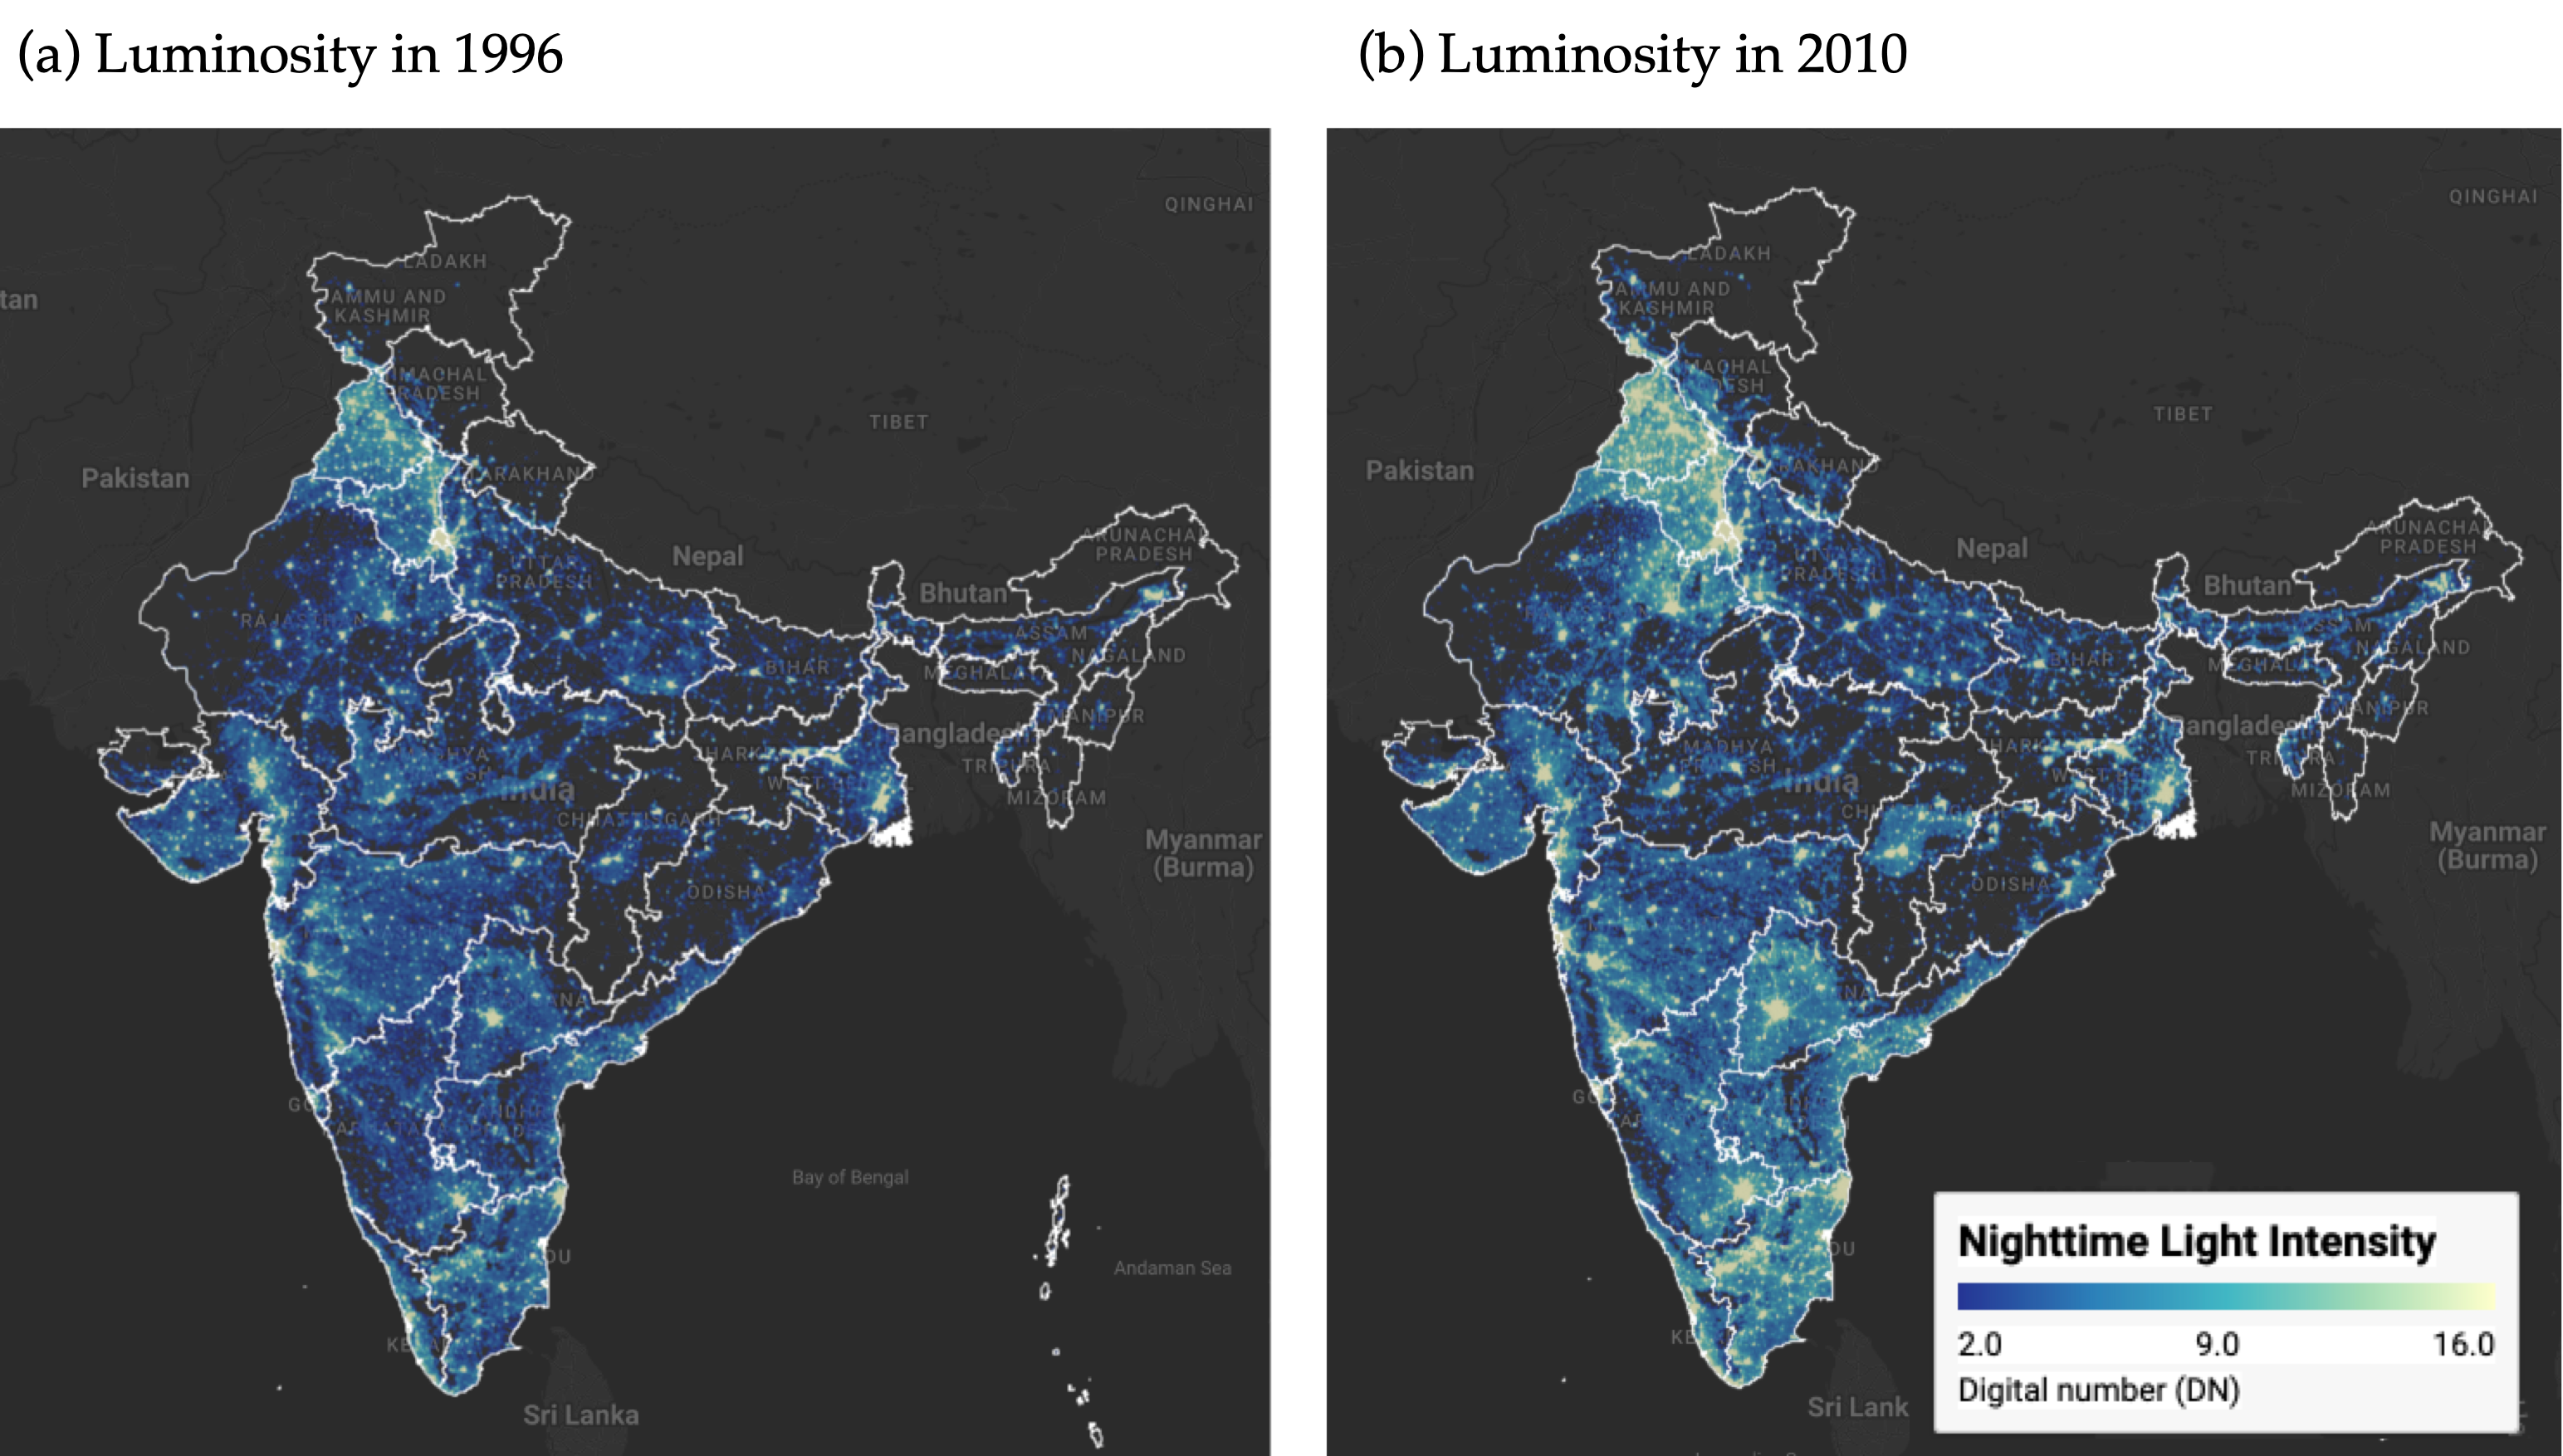
\includegraphics[keepaspectratio]{images/luminosity_map.png}}

}

\caption{\label{fig-map}Regional luminosity in India: 1996 vs 2010
Notes: Luminosity is measured in radiance-calibrated digital number (DN)
values from DMSP-OLS satellites. Interactive web application available
at \url{https://bit.ly/india-rc-ntl}. Source: Authors' visualization
using pre-processed luminosity images from the Earth Observation Group
(NOAA/NCEI). See
\href{https://quarcs-lab.github.io/project2025s-py/notebooks/c01_view_from_space.html}{View
from outer space} notebook for source code.}

\end{figure}%

Figure~\ref{fig-map} presents static maps of luminosity in the initial
and final years, 1996 and 2010, captured from our interactive
application. The maps show a noticeable increase in brightness across
most parts of India in 2010. Because nighttime lights serve as a proxy
for economic activity, this increase in luminosity reflects economic
growth over the period. Figure~\ref{fig-convergence} then illustrates
the relationship between per-capita growth in nighttime lights and
initial per-capita nighttime light. The scatterplot shows an inverse
relationship: the estimated \(\beta\)-convergence coefficient of about
\(-0.02\) implies an annual speed of convergence of roughly 2.3\% and a
half-life of about 30 years, consistent with the seminal finding of
\citet{barro_sala_convergence}.

\begin{figure}[H]

\centering{

\pandocbounded{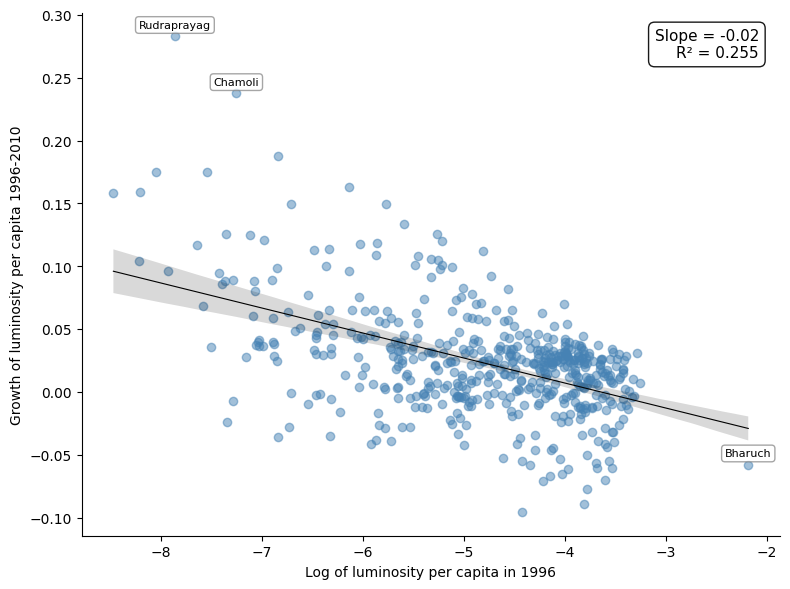
\includegraphics[keepaspectratio]{index_files/figure-latex/notebooks-c02_regional_convergence_sc-fig-convergence-output-1.png}}

}

\caption{\label{fig-convergence}Regional luminosity convergence across
districts in India Notes: Each point represents one of the 520
districts. The regression line shows the estimated beta-convergence
relationship. Outlier districts are labeled. Source: Data from Chanda
and Kabiraj (2020). See
\href{notebooks/c02_regional_convergence_sc.ipynb}{Regional convergence}
notebook for source code.}

\end{figure}%

Next, we examine case studies of three economically disadvantaged states
in India to illustrate their growth patterns over the study period.
Among these, Bihar is the poorest, with a per-capita income at 31.2\% of
the national average, while Uttar Pradesh and Chhattisgarh stand at
55.3\% and 59.9\% respectively.\footnote{The figures are relative per
  capita income for 2000--01, the census year closest to the start of
  our study period, measured as per capita net state domestic product
  divided by per capita net national income. They are taken from Table 4
  of Sanyal and Arora, ``Relative Economic Performance of Indian States:
  1960-61 to 2023-24'', Economic Advisory Council to the Prime Minister,
  Working Paper EAC-PM/WP/31/2024, September 2024.}
Figure~\ref{fig-map2} displays the change in luminosity in these three
states during our study period. Although these states remain among the
poorest, there is a noticeable increase in luminosity over the course of
the study.

\begin{figure}

\centering{

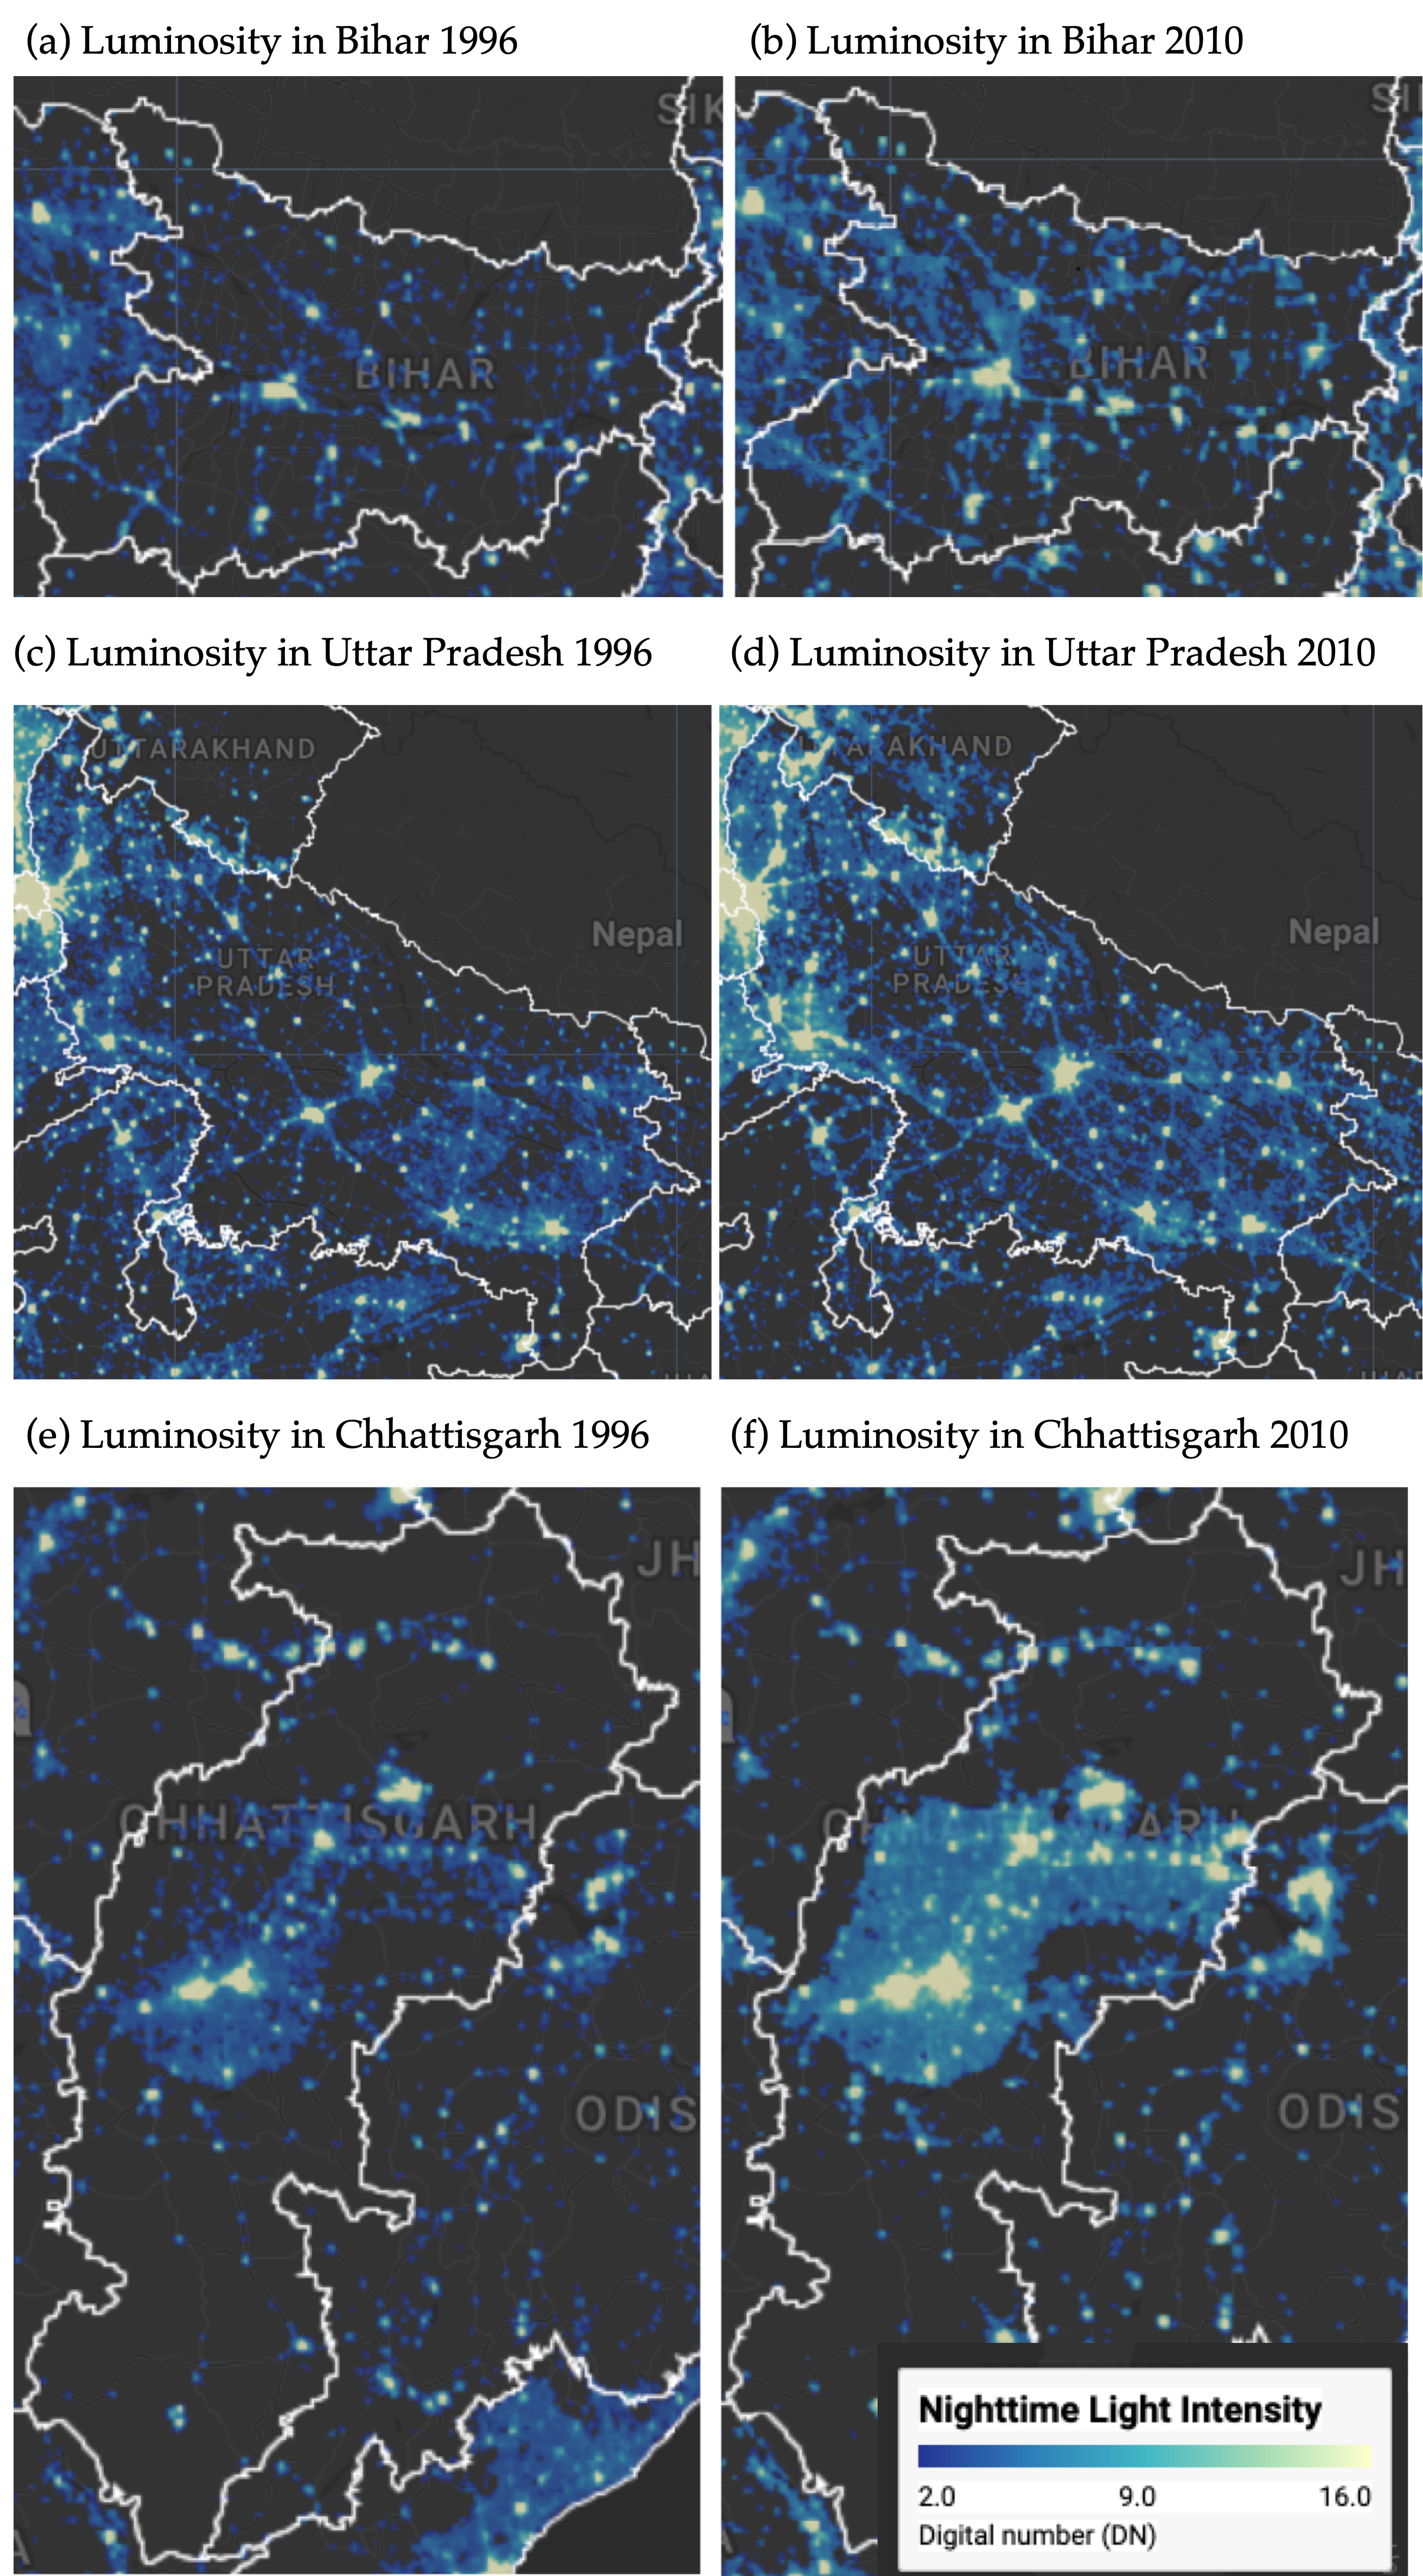
\includegraphics[width=0.75\linewidth,height=\textheight,keepaspectratio]{images/luminosity_map2.png}

}

\caption{\label{fig-map2}Some illustrative examples of regional
convergence Notes: Luminosity is measured in radiance-calibrated digital
number (DN) values from DMSP-OLS satellites. Interactive web application
available at \url{https://bit.ly/india-rc-ntl}. Source: Authors'
visualization using pre-processed luminosity images from the Earth
Observation Group (NOAA/NCEI). See
\href{https://quarcs-lab.github.io/project2025s-py/notebooks/c01_view_from_space.html}{View
from outer space} notebook for source code.}

\end{figure}%

\subsection{Spatial dependence is a feature of the convergence
process}\label{spatial-dependence-is-a-feature-of-the-convergence-process}

Before proceeding with the formal econometric analysis, we examine the
spatial distribution of the variables under study. Choropleth maps are a
natural tool for this purpose, because they show how a variable of
interest varies across geographic units and reveal patterns that summary
statistics alone would hide. Figure~\ref{fig-chorophleths} presents the
spatial distribution of initial luminosity in 1996 and of the subsequent
growth rate of luminosity over the 1996--2010 period across the 520
districts in our sample.

\begin{figure}[H]

\centering{

\pandocbounded{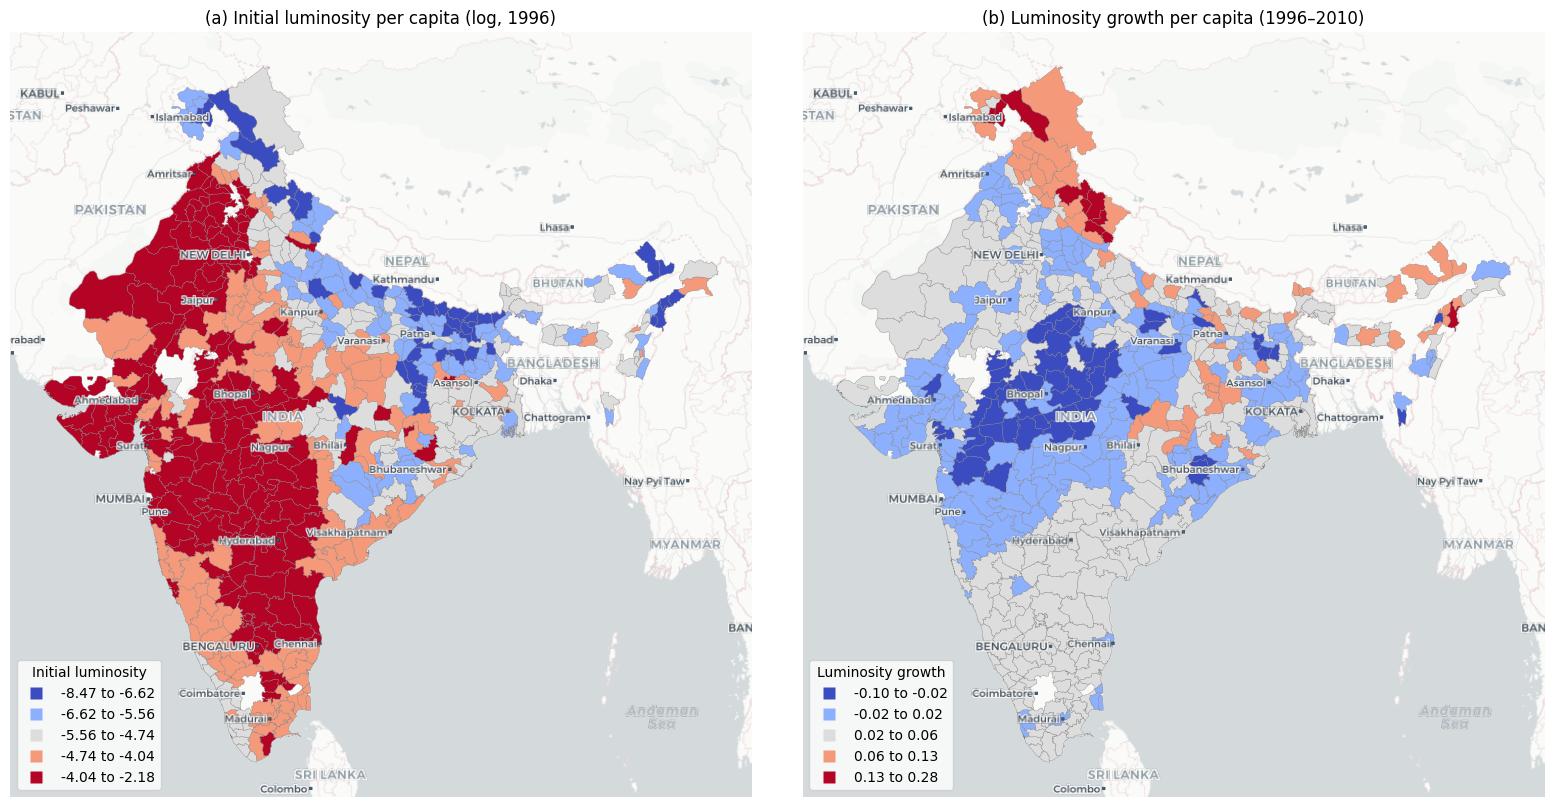
\includegraphics[keepaspectratio]{index_files/figure-latex/notebooks-c03_spatial_dependence_lisa-fig-chorophleths-output-1.png}}

}

\caption{\label{fig-chorophleths}Spatial distribution of initial
luminosity and luminosity growth Notes: Districts are classified into
five categories using Fisher-Jenks natural breaks. Panel (a) shows log
of luminosity per capita in 1996. Panel (b) shows luminosity growth per
capita over 1996--2010. Source: Data from Chanda and Kabiraj (2020). See
\href{notebooks/c03_spatial_dependence_lisa.ipynb}{Spatial dependence}
notebook for source code.}

\end{figure}%

The choropleth maps in Figure~\ref{fig-chorophleths} reveal a distinct
spatial pattern. Panel (a) shows that initial luminosity levels are
concentrated in specific geographic corridors, with higher values
clustered in western and north-western India, while large portions of
eastern and northern India exhibit markedly lower luminosity. Panel (b),
which displays the growth rate of luminosity per capita over the study
period, presents a pattern that is largely the inverse of the initial
distribution. Districts that were initially bright tend to exhibit lower
growth rates, whereas districts that were initially dim tend to grow at
a faster rate. This spatial inversion provides a first visual indication
that regional convergence in India may have an important spatial
dimension.

While the choropleth maps suggest the presence of spatial structure in
both variables, a formal analysis of spatial dependence requires a
definition of the neighborhood of each district. This neighborhood
structure is specified through a spatial weight matrix, which encodes
the connectivity between geographic units. In this study, we adopt a six
nearest neighbors weight matrix, so that for each of the 520 districts
the six nearest districts by centroid distance are identified as its
neighbors. This connectivity structure is visualized as a network in
Figure~\ref{fig-wmatrix6nn}, where each node represents a district
centroid and each edge connects a district to one of its six nearest
neighbors.

\begin{figure}[H]

\centering{

\pandocbounded{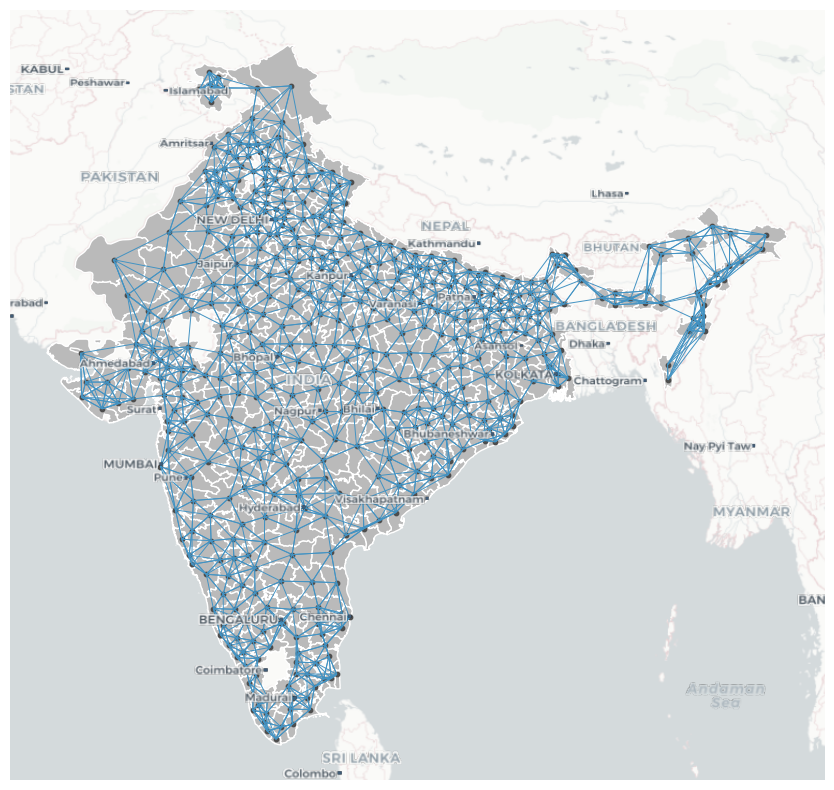
\includegraphics[keepaspectratio]{index_files/figure-latex/notebooks-c03_spatial_dependence_lisa-fig-wmatrix6nn-output-1.png}}

}

\caption{\label{fig-wmatrix6nn}Spatial connectivity structure based on
six nearest neighbors Notes: Each node represents a district centroid.
Each edge connects a district to one of its six geographically closest
neighbors. The weight matrix is row-standardized. Source: Data from
Chanda and Kabiraj (2020). See
\href{notebooks/c03_spatial_dependence_lisa.ipynb}{Spatial dependence}
notebook for source code.}

\end{figure}%

With the neighborhood of each district defined, we can formally assess
the degree of spatial dependence in the variables. Spatial dependence
can be understood through two complementary concepts: the overall degree
of clustering in the data, and the specific locations of statistically
significant clusters and spatial outliers. The Global Moran's I
statistic captures the first of these concepts. In our data, the Moran's
I for initial luminosity per capita is 0.73 (\(p = 0.001\)), which
indicates strong positive spatial autocorrelation: districts with high
(low) initial luminosity tend to be surrounded by districts that are
also bright (dim). The Moran's I for luminosity growth is 0.60
(\(p = 0.001\)), which confirms that the growth rates of neighboring
districts are also significantly correlated. Both the initial level and
the subsequent growth of luminosity therefore exhibit substantial
spatial clustering.

We now turn to the LISA statistics, which locate the significant
clusters and outliers behind these global measures.
Figure~\ref{fig-dependence-initial} presents the Moran scatterplot and
LISA cluster map for initial luminosity per capita. The cluster map
identifies distinct geographic concentrations. HH clusters mark the most
luminous regions and their bright neighbors, while LL clusters highlight
contiguous areas of low luminosity. These are predominantly in eastern
and northern India, in Bihar, eastern Uttar Pradesh, and Jharkhand,
together with the Himalayan north and the northeast.

\begin{figure}[H]

\centering{

\pandocbounded{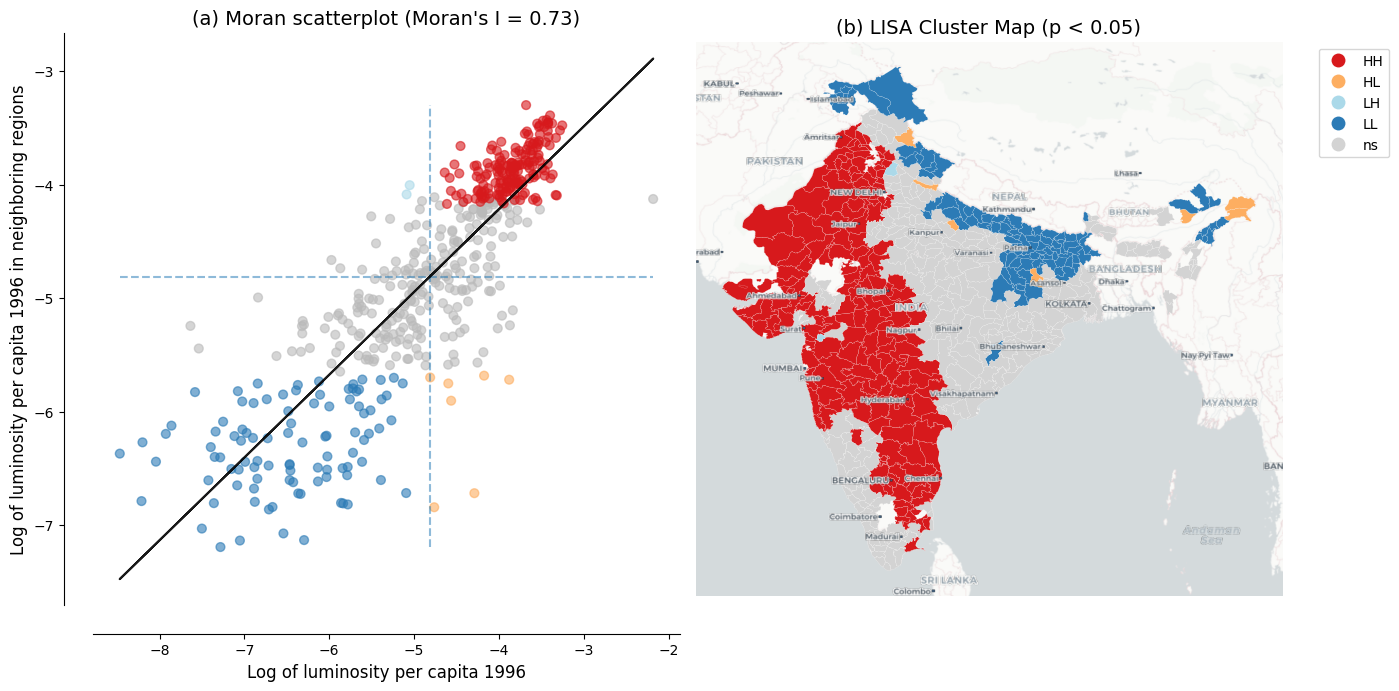
\includegraphics[keepaspectratio]{index_files/figure-latex/notebooks-c03_spatial_dependence_lisa-fig-dependence-initial-output-1.png}}

}

\caption{\label{fig-dependence-initial}Spatial dependence in the initial
level of luminosity Notes: Panel (a) shows the Moran scatterplot with
Global Moran's I statistic. Panel (b) shows the LISA cluster map with
statistically significant clusters at p \textless{} 0.05 based on 999
permutations. Source: Data from Chanda and Kabiraj (2020). See
\href{notebooks/c03_spatial_dependence_lisa.ipynb}{Spatial dependence}
notebook for source code.}

\end{figure}%

The same LISA analysis applied to luminosity growth rates reveals a
geographic pattern that is largely the inverse of the initial luminosity
clusters, as shown in Figure~\ref{fig-dependence-growth}. Districts that
formed HH clusters in initial luminosity tend to appear as LL clusters
in luminosity growth, and the dimmest clusters tend to emerge as HH
clusters in growth.\footnote{The initially prosperous areas therefore
  experienced relatively slower growth over the study period, while the
  initially lagging areas grew faster.} This spatial inversion between
the initial level and the subsequent growth of luminosity is the spatial
signature of the convergence process: red regions in the initial
luminosity map become blue regions in the growth map, and vice versa.
These local spatial patterns provide visual evidence that spatial
dependence is a prominent feature of the regional convergence process
observed in India, and they motivate the use of spatial econometric
methods.

\begin{figure}[H]

\centering{

\pandocbounded{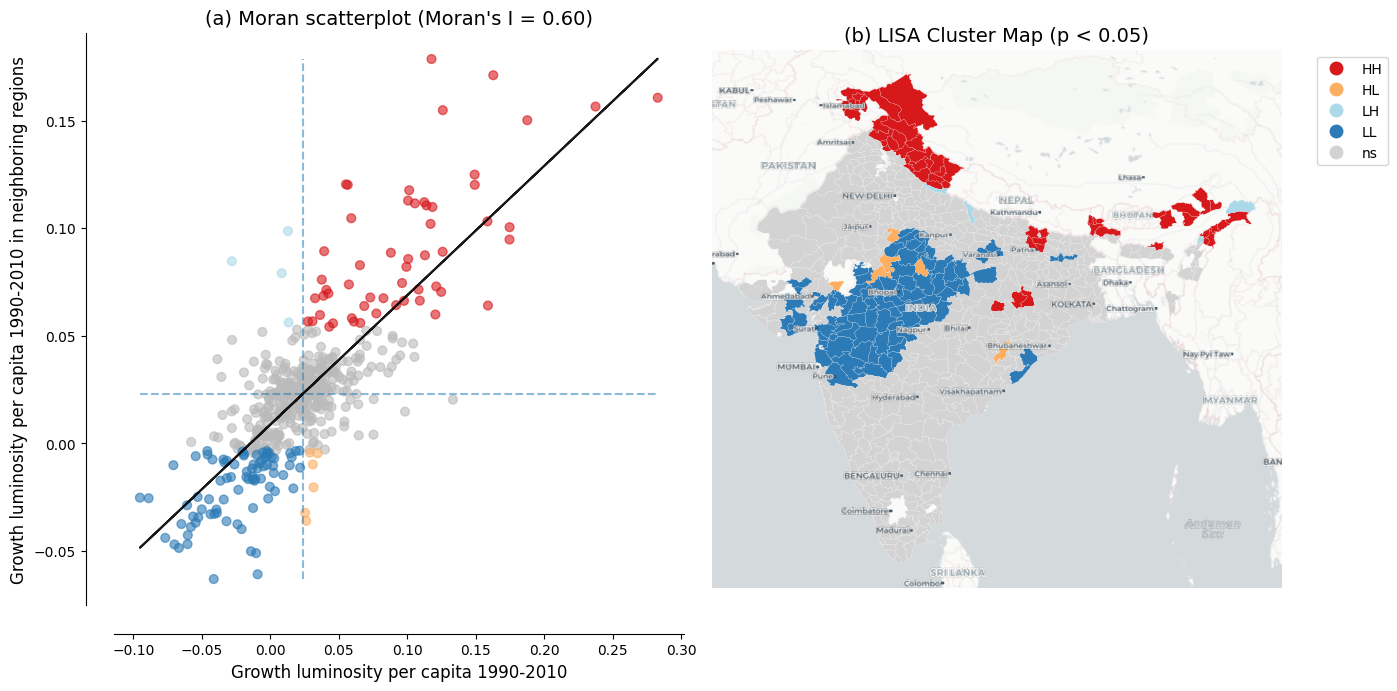
\includegraphics[keepaspectratio]{index_files/figure-latex/notebooks-c03_spatial_dependence_lisa-fig-dependence-growth-output-1.png}}

}

\caption{\label{fig-dependence-growth}Spatial dependence in the growth
rate of luminosity Notes: Panel (a) shows the Moran scatterplot with
Global Moran's I statistic. Panel (b) shows the LISA cluster map with
statistically significant clusters at p \textless{} 0.05 based on 999
permutations. Source: Data from Chanda and Kabiraj (2020). See
\href{notebooks/c03_spatial_dependence_lisa.ipynb}{Spatial dependence}
notebook for source code.}

\end{figure}%

\subsection{Evidence of spatial spillovers in regional
convergence}\label{evidence-of-spatial-spillovers-in-regional-convergence}

The regression results of Table~\ref{tbl-models} provide evidence of
both unconditional and conditional convergence across districts in
India. Both conventional ordinary least squares (OLS) and spatial
econometric approaches indicate significant negative relationships
between initial luminosity levels and subsequent growth rates. The
direct effects, which represent within-district convergence, remain
negative and of similar order across specifications, ranging from -0.020
to -0.026. This consistency across specifications and estimation methods
suggests that poorer districts are catching up to their wealthier
counterparts, even after controlling for district characteristics and
state-level fixed effects.

\begin{longtable}[]{@{}
  >{\raggedright\arraybackslash}p{(\linewidth - 16\tabcolsep) * \real{0.1282}}
  >{\raggedright\arraybackslash}p{(\linewidth - 16\tabcolsep) * \real{0.1154}}
  >{\raggedright\arraybackslash}p{(\linewidth - 16\tabcolsep) * \real{0.0897}}
  >{\raggedright\arraybackslash}p{(\linewidth - 16\tabcolsep) * \real{0.1154}}
  >{\raggedright\arraybackslash}p{(\linewidth - 16\tabcolsep) * \real{0.1154}}
  >{\raggedright\arraybackslash}p{(\linewidth - 16\tabcolsep) * \real{0.1154}}
  >{\raggedright\arraybackslash}p{(\linewidth - 16\tabcolsep) * \real{0.0897}}
  >{\raggedright\arraybackslash}p{(\linewidth - 16\tabcolsep) * \real{0.1154}}
  >{\raggedright\arraybackslash}p{(\linewidth - 16\tabcolsep) * \real{0.1154}}@{}}

\caption{\label{tbl-models}Unconditional and conditional convergence
across districts.}

\tabularnewline

\toprule\noalign{}
\begin{minipage}[b]{\linewidth}\raggedright
\end{minipage} & \begin{minipage}[b]{\linewidth}\raggedright
Model 1
\end{minipage} & \begin{minipage}[b]{\linewidth}\raggedright
\end{minipage} & \begin{minipage}[b]{\linewidth}\raggedright
Model 2
\end{minipage} & \begin{minipage}[b]{\linewidth}\raggedright
\end{minipage} & \begin{minipage}[b]{\linewidth}\raggedright
Model 3
\end{minipage} & \begin{minipage}[b]{\linewidth}\raggedright
\end{minipage} & \begin{minipage}[b]{\linewidth}\raggedright
Model 4
\end{minipage} & \begin{minipage}[b]{\linewidth}\raggedright
\end{minipage} \\
\midrule\noalign{}
\endhead
\bottomrule\noalign{}
\endlastfoot
& OLS & SDM & OLS & SDM & OLS & SDM & OLS & SDM \\
Direct & -0.020*** & -0.026*** & -0.022*** & -0.021*** & -0.025*** &
-0.026*** & -0.025*** & -0.025*** \\
& (0.002) & (0.002) & (0.003) & (0.002) & (0.003) & (0.002) & (0.003) &
(0.002) \\
Indirect & -- & 0.004 & -- & -0.001 & -- & -0.015* & -- & -0.013* \\
& & (0.006) & & (0.005) & & (0.009) & & (0.007) \\
Total & -0.020*** & -0.022*** & -0.022*** & -0.022*** & -0.025*** &
-0.041*** & -0.025*** & -0.037*** \\
& (0.002) & (0.006) & (0.003) & (0.005) & (0.003) & (0.009) & (0.003) &
(0.007) \\
Controls & No & No & No & No & Yes & Yes & Yes & Yes \\
State FE & No & No & Yes & Yes & No & No & Yes & Yes \\
AIC & -1945 & -2292 & -2409 & -2468 & -2211 & -2358 & -2465 & -2501 \\

\end{longtable}

The progression from unconditional to conditional specifications reveals
how the estimated convergence process is shaped by the inclusion of
additional covariates. In the OLS specifications, the direct effect is
-0.020 in Model 1 and -0.022 in Model 2, and it strengthens to -0.025
once district characteristics are added in Models 3 and 4. Omitting
these characteristics therefore attenuates the estimated speed of
convergence. The spatial Durbin direct effects match this pattern in the
conditional models, at -0.026 in Model 3 and -0.025 in Model
4.\footnote{The impact decomposition is unreliable in Model 1, where the
  spatial autoregressive parameter is very large, at about 0.80, which
  inflates the direct effect to -0.026. In Model 2 the indirect effect
  is indistinguishable from zero.} Once we account for structural
differences across districts, the underlying tendency for poorer
districts to catch up becomes more pronounced. State fixed effects
absorb unobserved state-level heterogeneity, such as differences in
governance and institutional quality, that might otherwise confound the
convergence relationship. They tighten the standard errors and moderate
the spatial total effect rather than strengthening it further.

The spatial Durbin model also reveals spatial spillover effects that are
not captured by traditional OLS estimations. These indirect effects,
which capture the influence of the initial conditions of neighboring
districts on the growth rate of a district, follow a notable pattern
across specifications. In the unconditional models (Models 1 and 2), the
estimated indirect effects are statistically insignificant and erratic,
negative in Model 2 but positive in Model 1.\footnote{Without controls,
  the strong residual spatial dependence confounds the spillover
  estimates with omitted variables.} Once district-level controls are
introduced (Models 3 and 4), the indirect effects become both larger in
magnitude and statistically significant at the 10\% level, reaching
-0.015 in Model 3 and -0.013 in our most comprehensive Model 4. The
spatial channels of convergence therefore become discernible only after
accounting for district-specific characteristics.

The total impact of initial conditions on growth, combining both direct
and spillover effects, is substantially larger when we account for
spatial dependence. In our fully specified model (Model 4), the total
convergence effect in the spatial Durbin model (-0.037) is approximately
51\% larger in magnitude than the OLS estimate (-0.025). Translated into
an annual speed of convergence, this raises the implied speed from about
3.0\% under OLS to about 5.2\% under the SDM, and it shortens the
implied half-life from roughly 23 to 13 years. The gap is even larger in
Model 3 (SDM total -0.041 against OLS -0.025, or 67\%), but the Model 3
and Model 4 spillover estimates are statistically indistinguishable, so
we anchor our interpretation on the preferred Model 4. These differences
indicate that in this setting conventional non-spatial approaches
understate the speed of regional convergence by failing to capture the
additional convergence channels created through spatial spillovers.

\begin{longtable}[]{@{}lllll@{}}

\caption{\label{tbl-speed}Implied annual speed of convergence and
half-life by model, from the OLS and SDM total effects of initial
luminosity.}

\tabularnewline

\toprule\noalign{}
Model & OLS speed & SDM speed & OLS half-life & SDM half-life \\
\midrule\noalign{}
\endhead
\bottomrule\noalign{}
\endlastfoot
Model 1 & 2.3\% & 2.6\% & 30 yr & 27 yr \\
Model 2 & 2.6\% & 2.7\% & 27 yr & 26 yr \\
Model 3 & 3.0\% & 6.2\% & 23 yr & 11 yr \\
Model 4 & 3.0\% & 5.2\% & 23 yr & 13 yr \\

\end{longtable}

Table~\ref{tbl-speed} reports the implied speeds and half-lives for all
four specifications. The spatial premium is concentrated in the
conditional models. In Models 1 and 2 the OLS and SDM speeds are nearly
identical, whereas in Models 3 and 4 the SDM raises the implied speed
from 3.0\% to 6.2\% and 5.2\%, shortening the half-life from 23 years to
11 and 13 years respectively.\footnote{The unconditional speeds are
  2.3\% against 2.6\% in Model 1 and 2.6\% against 2.7\% in Model 2.}

The model fit statistics further support the spatial econometric
approach. The Akaike Information Criterion (AIC) consistently favors the
spatial Durbin model over OLS across all four specifications, and the
most comprehensive model (Model 4 SDM) achieves the lowest AIC value of
-2501 compared to -2465 for the corresponding OLS.\footnote{The
  improvement from incorporating spatial structure is most pronounced in
  the unconditional specification, where the AIC drops by 347 units when
  moving from OLS to SDM in Model 1, reflecting the large amount of
  spatial dependence left unmodeled by ordinary regressions. Even in the
  fully specified model, where state fixed effects already absorb much
  of the spatial heterogeneity, the SDM retains a meaningful advantage.}
Overall, these results suggest that regional convergence in India
operates not only through district-specific factors but also through
spatial interactions between neighboring districts. In this setting,
ignoring these interactions leads to both underestimated convergence
speeds and inferior model performance.

A word of caution is in order about how the indirect effects should be
read. The spatial Durbin model identifies spatial dependence in reduced
form: it establishes that the growth of a district covaries with the
initial conditions of its neighbors, conditional on its own
characteristics, but it does not establish why. Several distinct
processes generate the same reduced-form pattern. Neighboring districts
share geographic and agro-climatic conditions. They are often governed
by the same state, and so inherit common institutional and policy
environments that our state fixed effects absorb only in part. They are
connected by infrastructure whose effects do not stop at administrative
boundaries. Any omitted determinant of growth that is itself spatially
clustered will also be absorbed into the spatial terms of the model. The
measurement issues discussed below point in the same direction, since
blooming spreads light across district boundaries and can raise the
apparent correlation between neighbors for reasons unrelated to economic
interaction. We therefore read the indirect effects as evidence that
spatial structure is a feature of the convergence process, and not as an
estimate of the causal effect of the conditions of one district on the
growth of another. Establishing which channels are at work, and whether
they are causal, would require research designs built for that purpose,
a point we return to in the discussion.

\subsection{How these estimates compare with the convergence
literature}\label{how-these-estimates-compare-with-the-convergence-literature}

The speeds reported above can be placed against three sets of
benchmarks. The first is other work on Indian districts using the same
proxy. \citet{beyer_yamada_district_banks} study district-level
convergence in India with nighttime lights for 2013--2019 and report an
absolute convergence rate of 2.4\% and a conditional rate of 3.7\%. Our
own non-spatial estimates, 2.3\% in the bivariate relationship and 3.0\%
in the conditional OLS specification, are close to these figures, even
though the two studies cover different periods and rely on different
generations of the sensor. That two independent applications of the same
measurement strategy recover similar non-spatial convergence rates is
reassuring about the proxy, and it locates our contribution in what the
spatial specification adds rather than in the baseline itself.

The second comparison is with convergence estimated from luminosity
elsewhere. \citet{basher_etal_bangladesh_lights} find absolute
convergence across the 64 districts of Bangladesh at 4.57\% per year,
implying a half-life of 15 years, which is close to the 5.2\% and 13
years implied by our preferred spatial model.
\citet{carrington_jimenez_ecuador_lights} report convergence across
Ecuadorian provinces at a speed approximating the 2\% benchmark.
\citet{kacou_africa_convergence}, using night-light-based inequality
proxies for 49 African countries, instead finds multiple equilibria in
within-country regional inequality, with high-inequality countries
showing no tendency to converge toward low-inequality ones. Read against
the wider regional literature, our non-spatial estimates sit near the
familiar 2\% regularity while the spatial estimates sit above
it.\footnote{The regularity is about 2\% per year across 1,528 regions
  in 83 countries \citep{gennaioli_etal_growth_regions}, and a similar
  figure across regions of the United States, Japan, and five European
  countries \citep{salaimartin_regional_cohesion}.} That regularity
should not be treated as a law: a meta-analysis of some 600 published
estimates concludes that it is misleading to speak of a natural
convergence rate, since estimates produced by different specifications
are drawn from different populations
\citep{abreu_etal_meta_convergence}. These comparisons therefore locate
our estimates rather than validate them.

The third comparison bears most directly on what this article adds. That
convergence estimates are sensitive to spatial dependence is well
established, but the direction in which allowing for it moves the
estimated speed is not. Our result, an implied speed that rises from
3.0\% to 5.2\% once the spatial structure is modeled, agrees with
\citet{diop_africa_spillovers}, who finds that the estimated speed
increases substantially in a spatial Durbin specification and concludes
that earlier estimates may have been considerably understated. Other
studies find the opposite. \citet{isla_castillo_etal_eu_cohesion} report
that allowing for spatial dependence lowers the estimated convergence
speeds of European regions, and
\citet{santos_marquez_etal_indonesia_spatial} conclude that neighbor
effects have slowed the pace of convergence across Indonesian districts.
Within India, \citet{lolayekar_mukhopadhyay_india_spatial} find that the
estimated impact of initial income across states is considerably smaller
once spatial dependence is taken into account, and that states diverge
rather than converge.

The arithmetic behind these differences is straightforward in our own
case. The indirect effect carries the same negative sign as the direct
effect, so the two reinforce one another and the total effect exceeds
the OLS coefficient in magnitude. Where the initial conditions of
neighbors enter with the opposite sign, or where the spatial terms
absorb variation that the non-spatial model had attributed to initial
luminosity, the same exercise reduces the estimated speed. The
substantive point is therefore not that spatial dependence matters,
which is already known, but that in this setting it works in the
direction of faster measured convergence. The contrast with Indian
states at a more aggregated level further suggests that the scale of
analysis is part of what determines the answer.

\subsection{Robustness to alternative spatial weight
matrices}\label{robustness-to-alternative-spatial-weight-matrices}

The spillover results above use a six-nearest-neighbor (6NN) spatial
weight matrix. To assess their sensitivity to this choice, we
re-estimate the preferred Model 4 under six alternative specifications
and compare them with the 6NN baseline. The alternatives are four- and
eight-nearest neighbors, queen and rook contiguity, and inverse distance
and inverse-distance-squared, the last two applied within a distance
band.

\begin{figure}[H]

\centering{

\pandocbounded{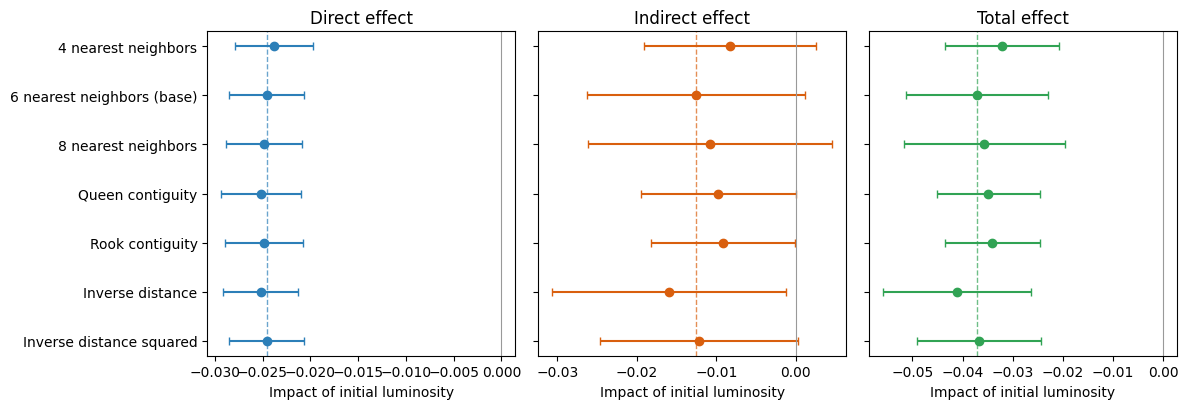
\includegraphics[keepaspectratio]{index_files/figure-latex/notebooks-c07_alternative_w_matrices-fig-altw-output-1.png}}

}

\caption{\label{fig-altw}Robustness of the Model 4 spatial impacts of
initial luminosity to the choice of spatial weight matrix. Points are
Direct, Indirect, and Total impacts; bars are 95\% Monte-Carlo
confidence intervals. The dashed lines mark the 6NN baseline estimates.}

\end{figure}%

\begin{longtable}[]{@{}
  >{\raggedright\arraybackslash}p{(\linewidth - 8\tabcolsep) * \real{0.3333}}
  >{\raggedright\arraybackslash}p{(\linewidth - 8\tabcolsep) * \real{0.1778}}
  >{\raggedright\arraybackslash}p{(\linewidth - 8\tabcolsep) * \real{0.2222}}
  >{\raggedright\arraybackslash}p{(\linewidth - 8\tabcolsep) * \real{0.1556}}
  >{\raggedright\arraybackslash}p{(\linewidth - 8\tabcolsep) * \real{0.1111}}@{}}

\caption{\label{tbl-altw}Model 4 spatial impacts of initial luminosity
under alternative spatial weight matrices (full LeSage--Pace method;
Monte-Carlo standard errors in parentheses).}

\tabularnewline

\toprule\noalign{}
\begin{minipage}[b]{\linewidth}\raggedright
Weight matrix
\end{minipage} & \begin{minipage}[b]{\linewidth}\raggedright
Direct
\end{minipage} & \begin{minipage}[b]{\linewidth}\raggedright
Indirect
\end{minipage} & \begin{minipage}[b]{\linewidth}\raggedright
Total
\end{minipage} & \begin{minipage}[b]{\linewidth}\raggedright
AIC
\end{minipage} \\
\midrule\noalign{}
\endhead
\bottomrule\noalign{}
\endlastfoot
4 nearest neighbors & -0.024***(0.002) & -0.008(0.006) &
-0.032***(0.006) & -2468 \\
6 nearest neighbors (base) & -0.025***(0.002) & -0.013*(0.007) &
-0.037***(0.007) & -2501 \\
8 nearest neighbors & -0.025***(0.002) & -0.011(0.008) &
-0.036***(0.008) & -2485 \\
Queen contiguity & -0.025***(0.002) & -0.010**(0.005) & -0.035***(0.005)
& -2463 \\
Rook contiguity & -0.025***(0.002) & -0.009**(0.005) & -0.034***(0.005)
& -2469 \\
Inverse distance & -0.025***(0.002) & -0.016**(0.007) & -0.041***(0.008)
& -2486 \\
Inverse distance squared & -0.025***(0.002) & -0.012*(0.006) &
-0.037***(0.006) & -2485 \\

\end{longtable}

The convergence spillovers are robust to the choice of spatial weights
(Figure~\ref{fig-altw} and Table~\ref{tbl-altw}). The direct
(within-district) convergence effect is essentially unchanged across all
seven specifications, ranging from -0.024 to -0.025 and always
significant at the 1\% level. The total convergence effect likewise
remains negative and significant throughout, ranging from -0.032 to
-0.041, with the 6NN baseline (-0.037) near the middle of this range.
The indirect (spillover) component is negative in every specification
and statistically significant under most of them. This stability
indicates that the direct and total convergence effects are not an
artifact of the particular neighbor definition. The spillover component
is negative throughout and significant under five of the seven, which is
a consistent if weaker pattern.

The results reported so far treat luminosity as a proxy for economic
output, which is the use that the convergence literature has made of it.
The discussion that follows asks first what the magnitude of these
estimates implies for regional policy, and what rests on the use of a
single growth period. It then turns to a second use of the same data,
since nighttime lights also record electrification, urbanization, and
broader socioeconomic conditions, and the reproducible workflow
assembled here can be pointed at those dimensions as readily as at
output. That possibility is pursued in an exploratory way, asking how
luminosity relates to cultural participation across Indian states.

\section{Discussion}\label{discussion}

\subsection{What the magnitude of the effects implies for regional
policy}\label{what-the-magnitude-of-the-effects-implies-for-regional-policy}

The difference between the two readings of Model 4 is large enough to
matter for policy. Under the OLS estimate, a district closes half of the
gap to its steady state in about 23 years; under the spatial Durbin
estimate, in about 13 years. Over the fourteen years of our sample, that
is the difference between closing roughly 34\% of the initial gap and
closing roughly 52\% of it. The first figure describes catch-up over a
generation, while the second describes catch-up within the horizon over
which development programs are designed, funded, and evaluated.

The distinction matters because it changes what can reasonably be
expected of an intervention. If convergence is slow, support for lagging
districts must be sustained across political cycles before its effects
become visible in aggregate outcomes, and the absence of visible
catch-up within the lifetime of a program is weak evidence that the
program has failed. If convergence is faster, as the spatial estimates
imply, the returns to a well-targeted intervention should appear within
a normal evaluation window, and the case for measuring them is
correspondingly stronger.

The results also speak to the level at which such policies should
operate. We find convergence across districts over 1996--2010, whereas
\citet{lolayekar_mukhopadhyay_india_spatial}, working with Indian states
over a longer period, find divergence. Catch-up that is visible at the
district level and absent at the state level is an argument for treating
the district as the unit of intervention, which is what the Aspirational
Districts Programme of India already does.\footnote{The programme was
  launched in 2018 to direct additional resources to the least developed
  districts of the country.} The spatial results add a qualification to
that logic: the growth of a district is associated with the initial
conditions of its neighbors, so a lagging district surrounded by other
lagging districts is in a different position from one adjacent to a
growing cluster, and a targeting rule that ranks districts one at a time
will not register that difference.

Spillovers, however, cut both ways, and the Indian evidence on
place-based policy is a caution as much as an encouragement.
\citet{hasan_etal_backward_districts} evaluate a tax-exemption program
for industrially backward districts and find that the resulting increase
in firm entry and employment was driven in part by the displacement of
activity from neighboring districts that narrowly missed qualifying, and
that the effects did not persist once the program ended. Activity moved
across a boundary would appear in our framework as a spatial
relationship between neighbors, and it is not the kind of spillover on
which a case for coordinated regional policy can be built. What the
satellite record does support is measurement: luminosity is responsive
enough to register a place-based package at this scale.\footnote{\citet{shenoy_place_based_policy}
  uses nighttime lights to evaluate a large place-based package in
  Uttarakhand and finds that luminosity rises sharply on the targeted
  side of the new state border, which shows that the outcome we study is
  responsive enough to register policy at this scale.}

These implications follow if the indirect effects reflect genuine
interaction between districts. As set out in the results, the
reduced-form evidence is consistent with that reading but does not
establish it. The policy conclusions above should therefore be read with
that qualification attached.

\subsection{The single growth period and what a panel would
require}\label{the-single-growth-period-and-what-a-panel-would-require}

The estimates reported above rest on a single growth period, and the
cost of that design should be stated plainly. Three things follow from
working with one long difference. It cannot trace how the rate of
convergence evolved within the period. It cannot establish whether the
spatial spillovers estimated above were stronger in some years than in
others, or whether they emerged only part-way through. And it cannot
separate long-run convergence from whatever was specific to these
fourteen years, which in India included the maturing of the post-1991
reforms.

These are real limitations and the dynamics they concern are important,
but they are beyond the scope of this article, whose purpose is to add a
spatial dimension to an existing cross-sectional result rather than to
replace it with a dynamic one. The immediate obstacle is the data. The
dataset we adopt from \citet{chanda_kabiraj_district_convergence} holds
radiance-calibrated luminosity at six dates between 1996 and 2010, but
district population is observed only at the decennial censuses.
Per-capita luminosity at the intermediate dates would therefore rest on
interpolated denominators. Over a single long difference that
interpolation affects only the two endpoints, whereas in a panel it
would enter every observation, and it would do so in the time dimension
that a panel exists to exploit.

The more interesting question is what such a panel would be worth, and
here two distinct problems compound. The first belongs to growth
econometrics and predates nighttime lights. Panel estimates of
convergence run far above cross-sectional ones:
\citet{caselli_etal_convergence_debate} obtain a rate near 10\% per year
using panel methods that instrument for endogenous regressors, against
the 2\% that cross-sections deliver. How to read that gap remains
contested.\footnote{\citet{barro_convergence_modernisation} argues that
  country fixed effects generate a misleadingly high convergence rate,
  and that combining post-1960 with post-1870 evidence returns a figure
  close to the conventional 2\%. Meta-analytic evidence finds that
  corrections for unobserved heterogeneity raise estimated convergence
  systematically \citep{abreu_etal_meta_convergence}.} A panel
specification would therefore not simply produce a better-identified
version of our estimate; it would produce an estimate of something
different, whose relation to the long-run rate is itself disputed.

The second problem is specific to the proxy, and it points the same way.
Luminosity discriminates differences across places considerably better
than changes over time
\citep{chen_nordhaus_viirs_crosssection, asher_shrug_india}.
Convergence, however, is a long-run process, so the horizon over which
it is measured determines whether lights carry the relevant signal at
all. Over fourteen years most of the identifying variation is
cross-sectional, which is the use that lights currently support best.
Over the annual intervals that make panel methods attractive, the ratio
of signal to measurement error in the light series falls sharply, so a
short-horizon panel would combine a specification whose estimates are
already hard to interpret with a proxy operating where it is weakest.
\citet{chakrabarty_mukherjee_covid_convergence} estimate district
convergence across the pandemic period, and how such estimates should be
read depends on how much of the short-run movement in lights reflects
output rather than measurement.

Our own view follows from this. If panel methods are to be applied to
convergence in luminosity, the periods compared should be long: a
sequence of non-overlapping long differences rather than a
high-frequency panel. Harmonized DMSP--VIIRS series
\citep{li_etal_harmonization} now make that feasible across roughly
three decades, and re-estimating this specification as such a sequence
is the most promising temporal extension of the analysis reported here.

\subsection{An exploratory extension: Luminosity and cultural
participation}\label{an-exploratory-extension-luminosity-and-cultural-participation}

Nighttime lights capture not just GDP but a composite of
electrification, urbanization, infrastructure, and broader socioeconomic
conditions
\citep{henderson_storeygard_weil_lights, mellander_etal_lights_gdp}.
This multi-dimensional nature invites exploration of how luminosity
relates to socioeconomic indicators beyond strictly economic output. In
this section, we examine the association between luminosity and cultural
participation patterns across Indian states.

A growing literature argues that regional cultural attitudes constitute
an independent factor in economic development, not merely a by-product
of income or institutions. In particular,
\citet{tubadji_cultural_entropy} applies the Culture-Based Development
framework, whose central claim is a directional one. Cultural attitudes
and the participation patterns that reveal them are treated as a factor
shaping local development, rather than as an outcome that development
produces. That direction is what distinguishes the framework from
accounts in which culture is a by-product of income, and it also marks
the limit of what the exercise below can establish.\footnote{A
  cross-sectional association is consistent with either direction, and
  with both operating at once. What it can do is establish that the two
  are related, and describe the form that relationship takes.}

For India, the National Sample Survey (NSS) 47th Round (July--December
1991) surveys household cultural participation. Following the
Culture-Based Development framework, we reduce these survey items to six
dimensions and aggregate them to state means.\footnote{The six
  dimensions are live cultural performance, cultural telecast
  (TV/media), socio-cultural participation, cultural heritage and
  religion, live cultural shows, and sports. They are extracted from the
  survey items by principal-components analysis. See the
  \href{https://quarcs-lab.github.io/project2025s-py/notebooks/c06_spatial_culture.html}{Spatial
  culture} notebook for details and extended analyses.} With nighttime
lights data for an adjacent period (1992) now available for 32 Indian
states and union territories, we can examine the extent to which
luminosity is associated with regional cultural patterns. This part of
the analysis uses the Consistent and Corrected Nighttime Lights series
rather than the radiance-calibrated composites used above, because it is
the product that covers 1992. Given the small sample size (N = 32) and
the potential leverage of small territories at the extremes of the
distribution on linear correlation measures, we report Spearman rank
correlations throughout this section. Figure~\ref{fig-culture-scatter}
presents the relationship between log nighttime lights per capita and
the two cultural dimensions that show statistically significant
associations.

\begin{figure}[H]

\centering{

\pandocbounded{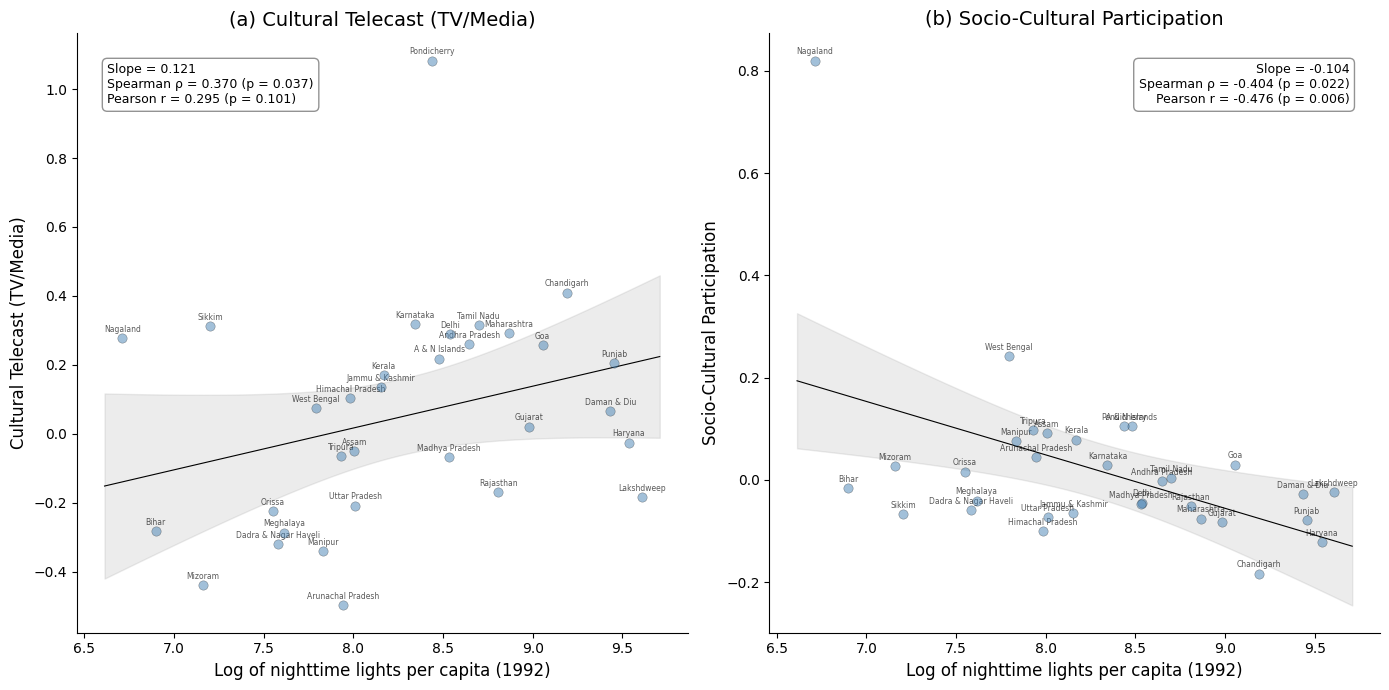
\includegraphics[keepaspectratio]{index_files/figure-latex/notebooks-c06_spatial_culture-fig-culture-scatter-output-1.png}}

}

\caption{\label{fig-culture-scatter}Relationship between nightlight
luminosity and cultural participation across 32 Indian states Notes:
Each point represents one of the 32 Indian states and union territories.
Panel (a) shows the bivariate relationship between log nighttime lights
per capita and cultural telecast (TV/media); Panel (b) shows the
relationship with socio-cultural participation. Solid line is the OLS
regression; gray band shows the 95\% confidence interval
(t-distribution, 30 df). Annotations report regression slope, Spearman
rank correlation, and Pearson correlation. Source: Nighttime lights from
CCNL DMSP-OLS (Zhao et al., 2022). Cultural participation from NSS 47th
Round (July--December 1991). See
\href{https://quarcs-lab.github.io/project2025s-py/notebooks/c06_spatial_culture.html}{Spatial
culture} notebook for source code.}

\end{figure}%

Cultural telecast (TV/media) exhibits a positive association with
nighttime light luminosity, with a Spearman rank correlation of 0.370
(\(p\) = 0.037). States with higher luminosity therefore consume more
culture through television and media. This link is intuitive, because
access to television depends on electrification and urbanization, which
are closely tied to luminosity.

In contrast, socio-cultural participation shows a significant negative
association, with a Spearman rank correlation of \$-\(0.404 (\)p\$ =
0.022). Community-based cultural engagement is therefore stronger in
states with less luminosity. This suggests that less urbanized regions
rely more on collective, in-person forms of cultural participation than
on media infrastructure.

Figure~\ref{fig-culture-lisa} presents the spatial distribution of these
two cultural variables through the lens of a LISA analysis. Both
dimensions exhibit significant spatial autocorrelation, which indicates
that cultural participation is not randomly distributed across Indian
states. The low-low cluster of cultural telecast in the northeast
coincides with the low-low cluster in the nighttime lights data,
although the high-high clusters of the two variables do not coincide.
The significant high-high cluster in cultural telecast is confined to
the southern states, while the northeastern states form a distinct
high-high cluster in community-based participation.

\begin{figure}[H]

\centering{

\pandocbounded{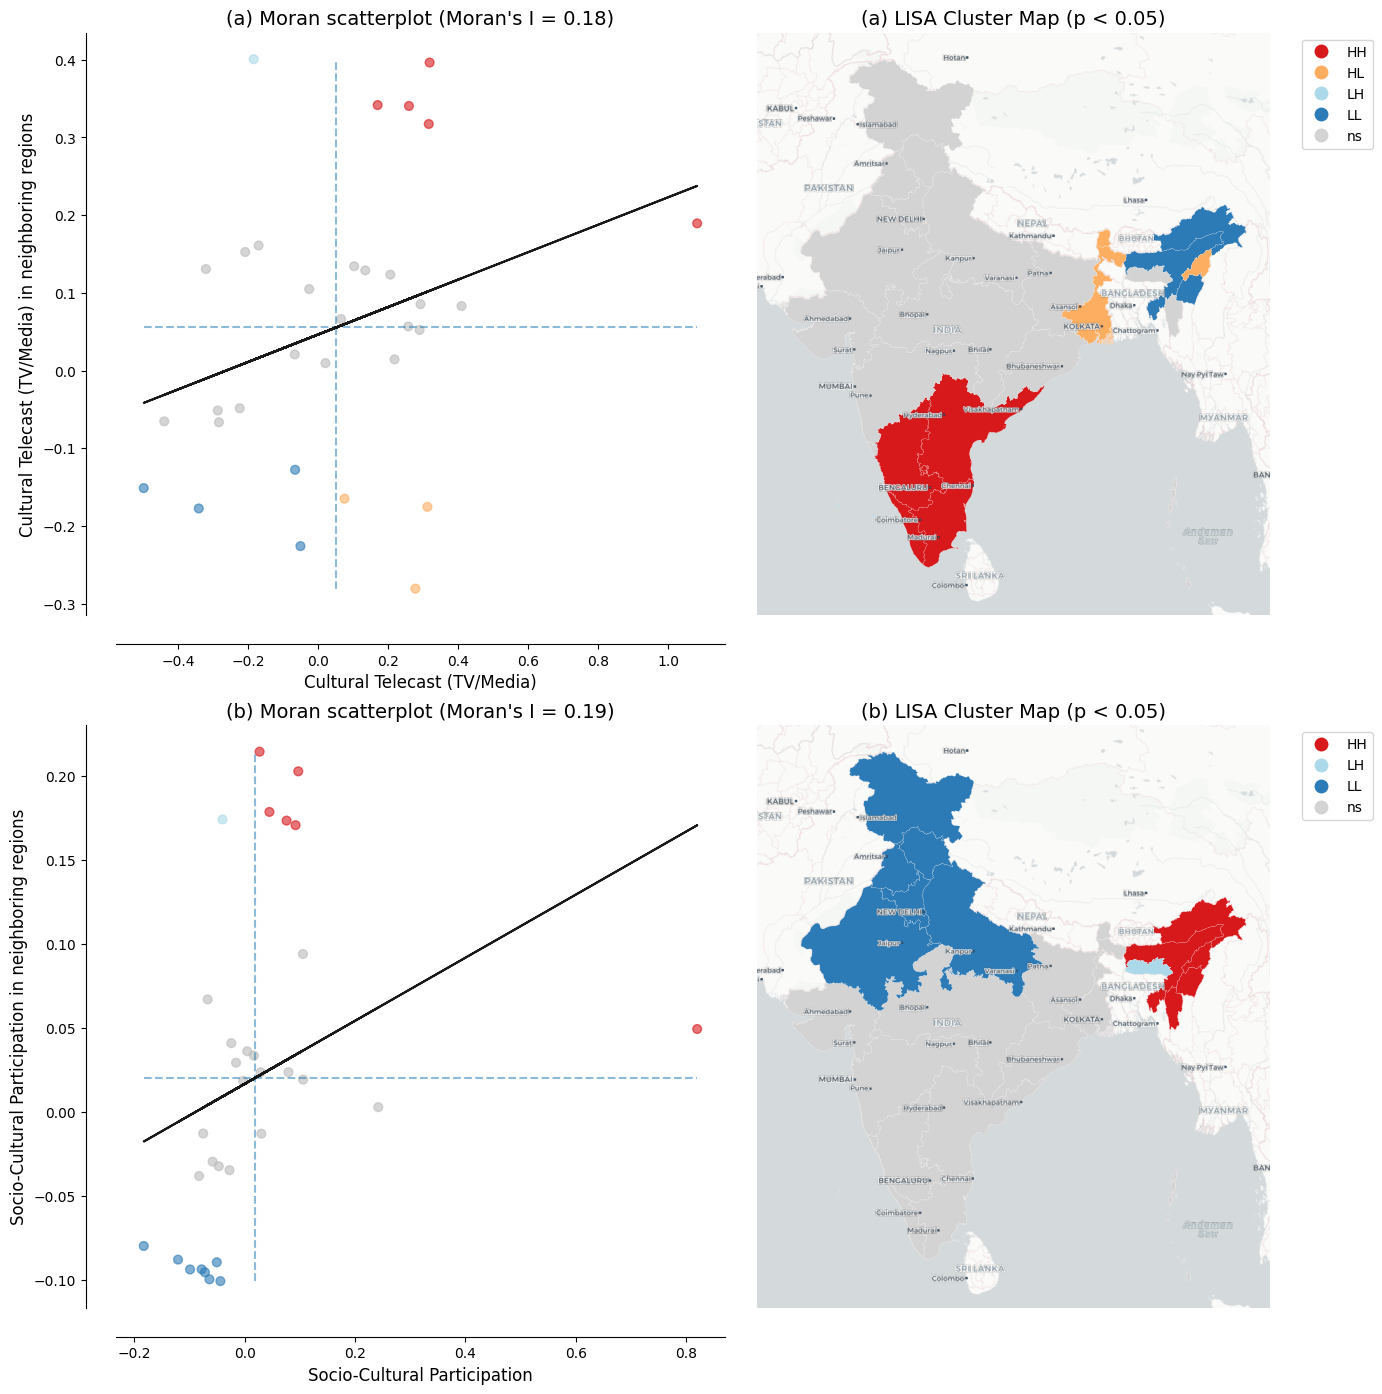
\includegraphics[keepaspectratio]{index_files/figure-latex/notebooks-c06_spatial_culture-fig-culture-lisa-output-1.png}}

}

\caption{\label{fig-culture-lisa}LISA cluster maps of cultural
participation across 32 Indian states Notes: Panel (a) shows results for
cultural telecast (TV/media); Panel (b) for socio-cultural
participation. Left subpanels show Moran scatterplots with the Global
Moran's I statistic. Right subpanels show LISA cluster maps with
statistically significant clusters at p \textless{} 0.05 based on 999
permutations and a 6-nearest-neighbors spatial weights matrix. Region
labels are overlaid from the CartoDB Positron basemap. Source: Cultural
participation data from NSS 47th Round (July--December 1991). See
\href{https://quarcs-lab.github.io/project2025s-py/notebooks/c06_spatial_culture.html}{Spatial
culture} notebook for source code.}

\end{figure}%

Together, these two results reveal a contrast in how regions engage with
culture: more luminous states favor media-based consumption, while less
luminous states sustain community-based participation. The remaining
four cultural dimensions show no statistically significant association
with luminosity. These findings rest on a small cross-section of 32
states observed at a single point in time, so larger datasets covering
more regions and periods would be needed to establish whether the
patterns are robust.

Two connections to the main analysis are worth drawing out, both offered
as interpretation rather than as findings. The first concerns what
luminosity measures. A positive association with media-based cultural
consumption and a negative one with community-based participation are
what one would expect if luminosity tracks electrification and
urbanization rather than economic output alone. The cultural results
are, in that sense, a small piece of evidence about the composite nature
of the proxy on which the convergence analysis rests, and they bear on
the measurement issues discussed below.

The second connection concerns spatial structure. Cultural participation
is not distributed randomly across states, since both dimensions
examined here are significantly spatially autocorrelated. Factors of
this kind, spatially clustered and correlated with development, are
precisely what a spatial Durbin model absorbs into its indirect effects
when they are not measured directly. We cannot test this with
state-level data for a single adjacent period, and we do not claim that
cultural participation drives the spillovers estimated in the results
section. What the exercise does is make concrete what a reduced-form
spatial model may be capturing, and it suggests that the Culture-Based
Development framework offers one route to testing the question directly,
should comparable data become available at the district level and over
time.

\subsection{New research directions}\label{new-research-directions}

Three kinds of gap limit what this literature can currently establish,
and each defines an agenda that the workflow used here is well placed to
support. The first two concern the raw material, namely the data
themselves and the geography those data cover. The third concerns the
range of theories those data have been used to test.

\subsubsection{Data gaps}\label{data-gaps}

Our analysis, following \citet{chanda_kabiraj_district_convergence},
relies on radiance-calibrated DMSP-OLS nighttime lights for 1996 to
2010, a dataset widely used as a proxy for economic activity
\citep{henderson_storeygard_weil_lights, chen_nordhaus_luminosity_gdp}.
DMSP-OLS is subject to well-documented limitations: top-coding in bright
urban cores, the absence of on-board calibration, and blooming artifacts
that spread light beyond its true source
\citep{gibson_etal_ntl_measurement, abrahams_etal_deblurring}. These are
not merely nuisances, and it is worth being explicit about how they bear
on our own estimates. Top-coding compresses variation at the bright end
of the distribution, which affects the recorded initial luminosity of
the most luminous districts. Two opposing biases follow: classical
measurement error in the regressor attenuates the convergence
coefficient toward zero, while measurement error in initial luminosity
that enters the growth rate with the opposite sign works in the
direction of overstating convergence. The net effect is ambiguous in
sign, and we do not claim to sign it. Measurement error is also unlikely
to be homogeneous across the sample, because the association between
luminosity and economic outcomes is stronger in urban than in rural
areas and Indian districts differ considerably in how urbanized they
are. Blooming has a clearer implication for the spillover estimates that
are central to this article. Because light spills across district
boundaries, part of what we measure as the luminosity of a district
originates with its neighbors, which mechanically raises the apparent
correlation between adjacent districts and could therefore inflate the
estimated indirect effects. That the direct and total effects hold
across all seven definitions of the neighborhood, and the indirect
effect under most of them (Table~\ref{tbl-altw}), shows they are not an
artifact of any particular neighbor definition, but it does not rule out
blooming; deblurring methods such as those of
\citet{abrahams_etal_deblurring} offer one route to addressing it
directly.

The Visible Infrared Imaging Radiometer Suite (VIIRS), operational since
2012, improves on DMSP-OLS in spatial resolution (roughly 750 meters
against 2.7 kilometers), in on-board radiometric calibration, and in
dynamic range, avoiding saturation in bright areas while detecting dim
lights in rural settlements
\citep{elvidge_etal_viirs, gibson_etal_ntl_measurement}. The
discontinuity between the DMSP (1992--2013) and VIIRS (2012--present)
sensor eras remains an obstacle to long-run work, which harmonization
efforts have begun to address \citep{li_etal_harmonization}, and recent
global series adjust explicitly for top-coding, blooming, and changes of
satellite system \citep{chiovelli_global_south}. Beyond better sensors,
combining lights with other satellite products improves measurement
where lights alone are weak.\footnote{Lights have been combined with
  daytime imagery for poverty prediction
  \citep{jean_etal_poverty_prediction}, with land cover in agricultural
  areas \citep{keola_etal_lights_poverty}, with multiple remote sensing
  indicators for subnational output
  \citep{chen_etal_turkey_viirs, hussein_etal_vietnam_ml}, and with
  survey data for multidimensional poverty
  \citep{theara_etal_cambodia_poverty}.} Applying such multi-source
approaches to Indian districts, and re-estimating our specification on
harmonized or VIIRS-era data, are the most immediate extensions of the
analysis reported here.

\subsubsection{Geographic gaps}\label{geographic-gaps}

A distinctive advantage of nighttime lights is that a single instrument
observes the entire planet under a common protocol, so that measurements
are comparable across countries and across regions in a way that
national accounts, compiled under different statistical systems and
capacities, are not \citep{henderson_storeygard_weil_lights}.
Comparability across settings and scales nevertheless requires explicit
adjustment \citep{chiovelli_global_south}. This global coverage is,
however, coverage of light rather than of economic activity, and the
distinction determines where the method works. Roughly one fifth of the
settlement footprint of the planet emits no radiance detectable from
space, and unlit settlements are concentrated in Africa, which accounts
for 39\% of them, rising to 65\% when only rural settlement areas are
considered \citep{mccallum_unlit_settlements}. Lights therefore measure
development that is illuminated: they track urban areas as they expand,
and rural areas as lighting infrastructure reaches them, but they are
close to silent where neither is happening. The empirical record matches
this description.\footnote{Across 34 sub-Saharan African countries the
  association between harmonized luminosity and household wealth is
  pronounced in urban areas and considerably weaker in rural ones
  \citep{jhamb_africa_nightlights}, and systematic assessments of which
  product to use, and where, reach similar conclusions
  \citep{gibson_etal_ntl_measurement}.}

The resulting gap is not simply that some regions have gone unstudied.
Regional inequality and convergence have been examined with luminosity
across 49 African countries \citep{kacou_africa_convergence}, as they
have across Chinese provinces \citep{glawe_mendez_china_luminosity},
Indonesian districts \citep{miranti_mendez_indonesia}, Thailand
\citep{tipayalai_mendez_thailand}, and Turkey
\citep{ursavas_mendez_turkey}. The gap is that the places where lights
carry the least information, rural and sparsely electrified areas, are
the same places where administrative statistics are weakest, which is
precisely where a satellite proxy would be most valuable. Closing it
calls less for further applications of the same proxy than for
validation against ground data in those settings, and for the
complementary sensors and multi-source methods described above.

\subsubsection{Theoretical gaps}\label{theoretical-gaps}

Within the convergence literature itself, our cross-sectional framework
documents an average effect and its spillover component but cannot
capture heterogeneity across the distribution. One direction is
distributional: methods designed for that purpose could reveal whether
Indian districts converge to a single steady state or form distinct
clubs, and combining them with spatial econometrics could expose spatial
poverty traps or growth poles that average estimates render invisible
\citep{rey_spatial_dynamics}.\footnote{The relevant tools are
  distribution dynamics \citep{quah_twin_peaks} and the regression-tree
  methods developed for identifying multiple growth regimes
  \citep{durlauf_johnson_convergence_clubs}.} A second direction
concerns identification: our spatial Durbin estimates capture spillovers
in reduced form without establishing whether they operate through
infrastructure linkages, labor migration, technology diffusion, or
market access, and quasi-experimental designs such as that of
\citet{asher_novosad_rural_roads} offer a route to isolating them.

Beyond convergence, luminosity is now used to study city size and urban
growth \citep{ch_martin_vargas_city_size}, electrification and the
provision of public goods \citep{min_etal_electrification}, and armed
conflict \citep{witmer_lights_conflict}. As in the exploratory extension
reported above, the same data can also be turned on socioeconomic
dimensions that are not economic output at all, such as the cultural
participation theorized by \citet{tubadji_cultural_entropy}. A rapidly
growing use is impact evaluation, in which lights measure the local
effect of a policy or a shock at fine spatial scales
\citep{bluhm_mccord_small_geographies}. Here a caveat is in order, and
it is one the literature has established rather than one we are
proposing. As noted above, lights discriminate differences across places
considerably better than changes over time.\footnote{VIIRS predicts
  cross-sectional GDP better than time-series GDP
  \citep{chen_nordhaus_viirs_crosssection}. In India, the elasticity of
  lights with respect to local outcomes is far lower in the time series
  than in the cross-section \citep{asher_shrug_india}. The relationship
  between lights and growth is also unstable across regions in both
  Brazil and India \citep{bickenbach_regional_gdp}.} The responsiveness
of lights to output also varies with baseline income, population
density, and sector \citep{bluhm_mccord_small_geographies}.\footnote{An
  evaluation may therefore fail to detect a real effect where lights
  react weakly, or attribute to a policy what is in fact heterogeneity
  in the relationship between light and output.} Evaluations over short
horizons that rest on luminosity therefore require validation against
local ground data before their estimates can be interpreted. The design
used here, a fourteen-year horizon, rests mostly on cross-sectional
variation, which is what lights currently support best.

Taken together, these three gaps describe a research agenda rather than
a list of caveats, and none of the work they imply requires starting
from scratch. The pipeline behind this article, running from the raw
satellite composites through the construction of the spatial weight
matrices to the impact decomposition and its robustness checks, is
public, documented, and executable in a browser. A reader who wants to
ask whether the patterns documented here hold in another country, in a
later period, under a different definition of the neighborhood, or for
an outcome other than economic output, can open the relevant notebook,
substitute their own data, and re-run it. The appearance of spatial
dependence in convergence processes across very different institutional
settings also suggests that the questions raised here are not specific
to India. That is the contribution we would most like this article to
make: not only an estimate of how quickly Indian districts converged
between 1996 and 2010, but a working template that lowers the cost of
asking the same question somewhere else.

\subsection{Research reproducibility and open
science}\label{research-reproducibility-and-open-science}

The complexity of satellite-based economic research, which involves
multi-step processing pipelines, spatial econometric estimation, and
geographic visualization, makes reproducibility both challenging and
essential. As \citet{donaldson_storeygard_remotesensing} note,
methodological choices in processing remotely sensed data, such as
sensor inter-calibration, can affect the empirical conclusions. The same
applies further down our own pipeline, at the construction of the
spatial weight matrix. Our own robustness analysis is a case in point:
the estimated convergence effects survive seven definitions of the
neighborhood, but that is something a reader can only confirm because
the code that produced each of them is available.

Open-source tools and cloud platforms are lowering the barriers to this
kind of verification. Cloud-based notebooks, such as those developed by
\citet{mendez_patnaik_notebook} for processing nighttime lights data,
remove the need for specialized local software. The combination of open
data, version-controlled code, and cloud execution makes the full
pipeline, from satellite imagery to econometric results, verifiable and
extensible by the broader research community.

\section{Concluding remarks}\label{concluding-remarks}

This article re-examines the regional convergence hypothesis across
Indian districts using satellite nighttime light data, interactive
visualizations, and spatial econometric modeling. Building on the work
of \citet{chanda_kabiraj_district_convergence}, we developed an
interactive web-based visualization tool, and our spatial
autocorrelation analyses indicate that spatial dependence is a notable
characteristic of both the satellite data and the regional convergence
process in India. Estimates from our spatial Durbin model indicate that
incorporating spatial spillovers increases the estimated speed of
regional convergence. The total convergence effect in our fully
specified model is approximately 51\% larger than conventional
non-spatial estimates, and the implied half-life of regional disparities
falls from roughly 23 years to 13. This finding suggests that in this
setting non-spatial convergence models understate the speed of regional
convergence, although the comparison with other regional literatures
shows that the direction of this adjustment is specific to the setting
rather than general. If the estimated indirect effects reflect genuine
spillovers, place-based development interventions would have broader
impacts than conventional estimates suggest, since their benefits would
reach neighboring districts as well as the districts they target. If
instead they partly reflect activity displaced across district
boundaries, as the evaluation literature on Indian place-based programs
cautions, the same estimates would overstate what those interventions
add in aggregate.

Our results also demonstrate the usefulness of satellite nighttime
lights for studying economic dynamics in countries where subnational
data are scarce, infrequent, or unreliable. Conventional economic
statistics at the district level are often unavailable or inconsistent
across administrative boundaries, especially in large developing
economies. Radiance-calibrated nighttime light data allowed us to
analyze 520 Indian districts at a spatial granularity that would be
difficult to achieve with traditional national accounts. This
data-driven approach is potentially transferable to other data-poor
contexts across the developing world, and the ongoing transition from
DMSP-OLS to the higher-resolution VIIRS sensor should yield more precise
measurement of subnational economic activity in future studies.

This study also shows how reproducible open-science practices can
strengthen the credibility and reach of scientific research. The entire
analytical pipeline is documented in Jupyter notebooks written in
Python, and the results are embedded within the manuscript through the
Quarto publishing framework.\footnote{A single manuscript source
  generates multiple output formats. The HTML version allows readers to
  engage with interactive visualizations, inspect the code of the
  computational notebooks, and re-evaluate the results in light of their
  source code.} By hosting the complete codebase and data in a public
GitHub repository, and by making the Python notebooks executable in the
cloud through Google Colaboratory, we aim to encourage broader adoption
of reproducible open-science practices. Section 4 sets out where we
believe the most valuable work now lies, in better data, in the regions
this method currently serves least well, and in the questions beyond
convergence that it is able to address. The materials accompanying this
article are meant to make starting on any of them straightforward.

\section{Acknowledgments}\label{acknowledgments}

This research project was supported by JSPS KAKENHI Grant Number
24K04884. During the preparation of this manuscript, the authors
acknowledge the use of Claude Code (Anthropic) to assist with manuscript
editing, computational notebook development, and research infrastructure
setup. After using this AI tool, the authors reviewed the outputs,
confirmed their accuracy, and take full responsibility for the content
of this publication.

\section{Conflict of Interest}\label{conflict-of-interest}

The authors declare no conflict of interest.

\section{Data and Code Availability}\label{data-and-code-availability}

All data and computational code used in this study are available in the
project repository at
\url{https://github.com/quarcs-lab/project2025s-py}. The interactive
HTML version of this manuscript
(\url{https://quarcs-lab.github.io/project2025s-py/}) embeds the
computational notebooks, allowing readers to inspect the complete
analytical pipeline from raw data to published results. Every analytical
notebook can be executed in the cloud using Google Colaboratory without
any local software installation: readers open the notebook and run it,
and the results, figures, and tables of this article are regenerated
from the raw data. The computational notebooks are implemented entirely
in Python. An earlier implementation of the same analysis used R and
Stata, and the present Python results are largely consistent with it.
The impact decomposition of the unconditional spatial Durbin model
(Model 1) differs, although its total effect is unchanged, and the AIC
values differ by a few units. The interactive Earth Engine application
linked in the text is a convenience layer for visualizing the underlying
imagery; its source code is included in the first notebook, and none of
the results reported in this article depend on it.


\bibliography{references.bib}



% This is the COPYRIGHT statement for the article.
\vspace*{\fill}
\tabcolsep0mm
\noindent
\begin{tabular*}{\textwidth}{ll}
	\toprule
	\multirow{2}{19mm}{
\includegraphics[width=18mm,height=10mm]{_extensions/region-ersa/REGION/CC-BY-88x31}} & {\small \multirow{2}{328pt}{\textcopyright\  by the authors. Licensee: REGION -- The Journal of ERSA, European Regional Science Association, Louvain-la-Neuve, Belgium. This article is distri-}} \\
	& \\[-1pt]
	\multicolumn{2}{l}{\small \multirow{2}{\textwidth}{buted under the terms and conditions of the Creative Commons Attri\-bution (CC BY) license (\href{http://creativecommons.org/licenses/by/4.0/}{http://creativecommons.org/licenses/by/4.0/}).}}\\
	& \\
	\bottomrule
\end{tabular*}

\end{document}
